\documentclass{article}\usepackage[]{graphicx}\usepackage[]{color}
% maxwidth is the original width if it is less than linewidth
% otherwise use linewidth (to make sure the graphics do not exceed the margin)
\makeatletter
\def\maxwidth{ %
  \ifdim\Gin@nat@width>\linewidth
    \linewidth
  \else
    \Gin@nat@width
  \fi
}
\makeatother

\definecolor{fgcolor}{rgb}{0.345, 0.345, 0.345}
\newcommand{\hlnum}[1]{\textcolor[rgb]{0.686,0.059,0.569}{#1}}%
\newcommand{\hlstr}[1]{\textcolor[rgb]{0.192,0.494,0.8}{#1}}%
\newcommand{\hlcom}[1]{\textcolor[rgb]{0.678,0.584,0.686}{\textit{#1}}}%
\newcommand{\hlopt}[1]{\textcolor[rgb]{0,0,0}{#1}}%
\newcommand{\hlstd}[1]{\textcolor[rgb]{0.345,0.345,0.345}{#1}}%
\newcommand{\hlkwa}[1]{\textcolor[rgb]{0.161,0.373,0.58}{\textbf{#1}}}%
\newcommand{\hlkwb}[1]{\textcolor[rgb]{0.69,0.353,0.396}{#1}}%
\newcommand{\hlkwc}[1]{\textcolor[rgb]{0.333,0.667,0.333}{#1}}%
\newcommand{\hlkwd}[1]{\textcolor[rgb]{0.737,0.353,0.396}{\textbf{#1}}}%
\let\hlipl\hlkwb

\usepackage{framed}
\makeatletter
\newenvironment{kframe}{%
 \def\at@end@of@kframe{}%
 \ifinner\ifhmode%
  \def\at@end@of@kframe{\end{minipage}}%
  \begin{minipage}{\columnwidth}%
 \fi\fi%
 \def\FrameCommand##1{\hskip\@totalleftmargin \hskip-\fboxsep
 \colorbox{shadecolor}{##1}\hskip-\fboxsep
     % There is no \\@totalrightmargin, so:
     \hskip-\linewidth \hskip-\@totalleftmargin \hskip\columnwidth}%
 \MakeFramed {\advance\hsize-\width
   \@totalleftmargin\z@ \linewidth\hsize
   \@setminipage}}%
 {\par\unskip\endMakeFramed%
 \at@end@of@kframe}
\makeatother

\definecolor{shadecolor}{rgb}{.97, .97, .97}
\definecolor{messagecolor}{rgb}{0, 0, 0}
\definecolor{warningcolor}{rgb}{1, 0, 1}
\definecolor{errorcolor}{rgb}{1, 0, 0}
\newenvironment{knitrout}{}{} % an empty environment to be redefined in TeX

\usepackage{alltt}
\usepackage[sc]{mathpazo}
\renewcommand{\sfdefault}{lmss}
\renewcommand{\ttdefault}{lmtt}
\usepackage[T1]{fontenc}
\usepackage{geometry}
\geometry{verbose,tmargin=2.5cm,bmargin=2.5cm,lmargin=2.5cm,rmargin=2.5cm}
\setcounter{secnumdepth}{2}
\setcounter{tocdepth}{2}
\usepackage[unicode=true,pdfusetitle,
 bookmarks=true,bookmarksnumbered=true,bookmarksopen=true,bookmarksopenlevel=2,
 breaklinks=false,pdfborder={0 0 1},backref=false,colorlinks=false]
 {hyperref}
\hypersetup{
 pdfstartview={XYZ null null 1}}

\makeatletter
%%%%%%%%%%%%%%%%%%%%%%%%%%%%%% User specified LaTeX commands.
\renewcommand{\textfraction}{0.05}
\renewcommand{\topfraction}{0.8}
\renewcommand{\bottomfraction}{0.8}
\renewcommand{\floatpagefraction}{0.75}

\makeatother
\IfFileExists{upquote.sty}{\usepackage{upquote}}{}
\begin{document}



\title{}



\maketitle
The results below are generated from an R script.

\begin{knitrout}
\definecolor{shadecolor}{rgb}{0.969, 0.969, 0.969}\color{fgcolor}\begin{kframe}
\begin{alltt}
\hlcom{###########################}
\hlcom{# Taylor Last}
\hlcom{# STAT 4350 FINAL PROJECT}
\hlcom{###########################}
\hlkwd{library}\hlstd{(ggplot2)}
\hlkwd{library}\hlstd{(rjags)}
\hlkwd{setwd}\hlstd{(}\hlstr{'/Users/taylorlast/Documents/UGA_FourthYear/STAT_4350/Final Project'}\hlstd{)}
\hlstd{baseball} \hlkwb{=} \hlkwd{read.csv}\hlstd{(}\hlstr{'baseball.csv'}\hlstd{)}

\hlcom{#####################################################################}
\hlcom{## Hierarchical linear model with team-specific random intercept   ##}
\hlcom{##                                                                 ##}
\hlcom{#####################################################################}
\hlcom{## Load team covariates}
\hlkwd{attach}\hlstd{(baseball)}
\end{alltt}


{\ttfamily\noindent\itshape\color{messagecolor}{\#\# The following objects are masked from baseball (pos = 3):\\\#\# \\\#\#\ \ \ \  BABIP, ERA., HR.9, K.BB., LOB., Name, Team, WAR, WHIP, WIN., X}}

{\ttfamily\noindent\itshape\color{messagecolor}{\#\# The following objects are masked from baseball (pos = 7):\\\#\# \\\#\#\ \ \ \  BABIP, ERA., HR.9, K.BB., LOB., Name, Team, WAR, WHIP, WIN., X}}

{\ttfamily\noindent\itshape\color{messagecolor}{\#\# The following objects are masked from baseball (pos = 10):\\\#\# \\\#\#\ \ \ \  BABIP, ERA., HR.9, K.BB., LOB., Name, Team, WAR, WHIP, WIN., X}}\begin{alltt}
\hlcom{## More exploratory data analysis}
\hlcom{# By team denomination}
\hlkwd{ggplot}\hlstd{(}\hlkwc{data}\hlstd{=baseball,}\hlkwd{aes}\hlstd{(}\hlkwc{x}\hlstd{=Team,}\hlkwc{y}\hlstd{=ERA.))}\hlopt{+}
  \hlkwd{geom_boxplot}\hlstd{()}\hlopt{+}
  \hlkwd{theme}\hlstd{(}\hlkwc{axis.text.x} \hlstd{=} \hlkwd{element_text}\hlstd{(}\hlkwc{angle} \hlstd{=} \hlnum{90}\hlstd{,} \hlkwc{vjust} \hlstd{=} \hlnum{1}\hlstd{,} \hlkwc{hjust} \hlstd{=} \hlnum{1}\hlstd{),}\hlkwc{plot.title} \hlstd{=} \hlkwd{element_text}\hlstd{(}\hlkwc{hjust} \hlstd{=} \hlnum{0.5}\hlstd{))}\hlopt{+}
  \hlkwd{ggtitle}\hlstd{(}\hlstr{'ERA adjusted by team'}\hlstd{)}
\end{alltt}
\end{kframe}

{\centering 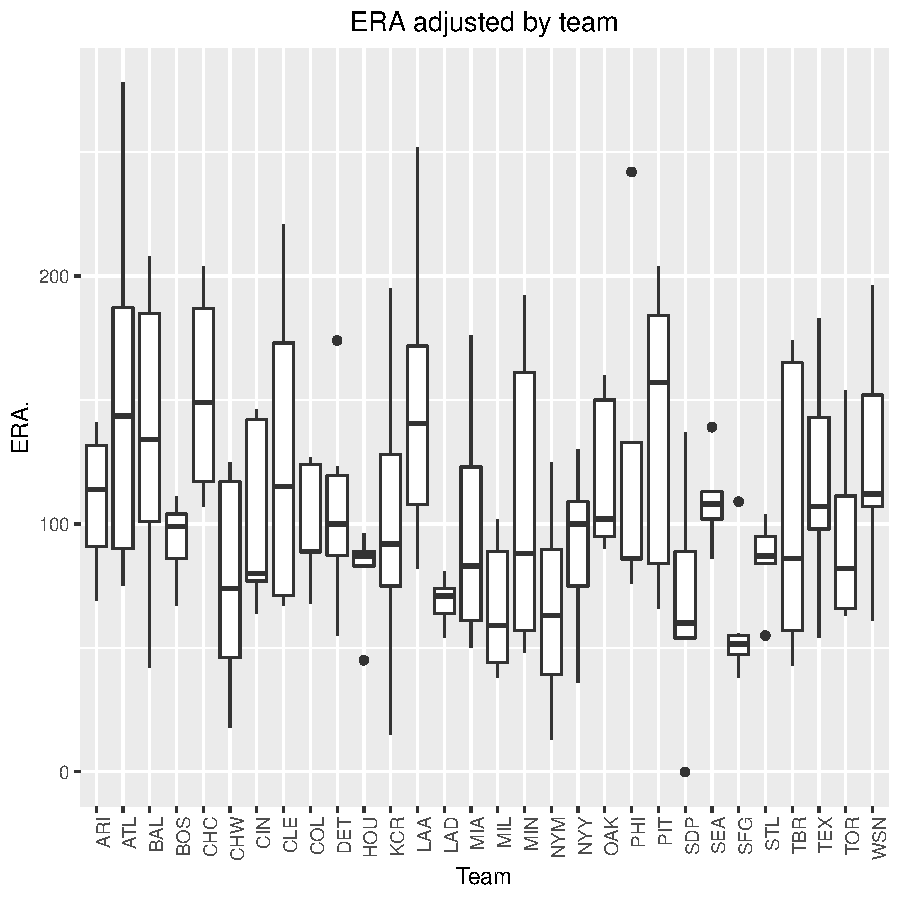
\includegraphics[width=.6\linewidth]{figure/FinalRFile-4350-Rnwauto-report-1} 

}


\begin{kframe}\begin{alltt}
\hlstd{n} \hlkwb{=} \hlkwd{dim}\hlstd{(baseball)[}\hlnum{1}\hlstd{]}
\hlstd{p} \hlkwb{=} \hlkwd{dim}\hlstd{(baseball)[}\hlnum{2}\hlstd{]} \hlopt{-} \hlnum{3}
\hlstd{n.teams} \hlkwb{=} \hlkwd{length}\hlstd{(}\hlkwd{unique}\hlstd{(Team))}

\hlstd{team_list} \hlkwb{=} \hlkwd{as.factor}\hlstd{(Team)}

\hlcom{## (1) Create data list}
\hlstd{dataList} \hlkwb{<-} \hlkwd{list}\hlstd{(}
  \hlstr{"n"} \hlstd{= n,}
  \hlstr{"p"} \hlstd{= p,}
  \hlstr{"n.teams"} \hlstd{= n.teams,}
  \hlstr{"Y"} \hlstd{= ERA.,}
  \hlstr{"HR9"} \hlstd{= HR.9,}
  \hlstr{"BABIP"} \hlstd{= BABIP,}
  \hlstr{"LOB"} \hlstd{= LOB.,}
  \hlstr{"WAR"} \hlstd{= WAR,}
  \hlstr{"KBB"} \hlstd{= K.BB.,}
  \hlstr{"WHIP"} \hlstd{= WHIP,}
  \hlstr{"WIN"} \hlstd{= WIN.,}
  \hlstr{"Team"} \hlstd{=} \hlkwd{as.factor}\hlstd{(Team))}

\hlcom{## (2) Specify list of parameter(s) to be monitored}
\hlstd{parameters} \hlkwb{<-} \hlkwd{c}\hlstd{(}\hlstr{"alpha"}\hlstd{,}\hlstr{"beta"}\hlstd{,}\hlstr{"sig2"}\hlstd{,}\hlstr{"sig2.alpha"}\hlstd{,}\hlstr{"icc"}\hlstd{)}

\hlcom{## (3) Specify initial values for parameter(s) in Metropolis-Hastings algorithm}
\hlstd{initsValues} \hlkwb{<-} \hlkwd{list}\hlstd{(}
  \hlstr{"alpha"} \hlstd{=} \hlkwd{rep}\hlstd{(}\hlnum{0}\hlstd{,n.teams),}
  \hlstr{"beta"} \hlstd{=} \hlkwd{rep}\hlstd{(}\hlnum{0}\hlstd{,p),}
  \hlstr{"tau2"} \hlstd{=} \hlnum{1}\hlstd{,}
  \hlstr{"tau2.alpha"} \hlstd{=} \hlnum{1}
\hlstd{)}

\hlcom{## (4) Specify parameters for running Metropolis-Hastings algorithm}
\hlstd{adaptSteps} \hlkwb{<-} \hlnum{10000}              \hlcom{# number of steps to "tune" the samplers}
\hlstd{burnInSteps} \hlkwb{<-} \hlnum{20000}             \hlcom{# number of steps to "burn-in" the samplers}
\hlstd{nChains} \hlkwb{<-} \hlnum{3}                    \hlcom{# number of chains to run}
\hlstd{numSavedSteps} \hlkwb{<-} \hlnum{50000}          \hlcom{# total number of steps in chains to save}
\hlstd{thinSteps} \hlkwb{<-} \hlnum{10}                  \hlcom{# number of steps to "thin" (1 = keep every step)}
\hlstd{nIter} \hlkwb{<-} \hlkwd{ceiling}\hlstd{((numSavedSteps}\hlopt{*}\hlstd{thinSteps)}\hlopt{/}\hlstd{nChains)}     \hlcom{# steps per chain}

\hlcom{## (5) Create, initialize, and adapt the model}
\hlcom{# This will require you to create a separate .txt file which specifies}
\hlcom{# the model}
\hlstd{jagsModel} \hlkwb{<-} \hlkwd{jags.model}\hlstd{(}\hlstr{"baseball.txt"}\hlstd{,}
                         \hlkwc{data} \hlstd{= dataList,}
                         \hlkwc{inits} \hlstd{= initsValues,}
                         \hlkwc{n.chains} \hlstd{= nChains,}
                         \hlkwc{n.adapt} \hlstd{= adaptSteps)}
\end{alltt}
\begin{verbatim}
## Compiling model graph
##    Resolving undeclared variables
##    Allocating nodes
## Graph information:
##    Observed stochastic nodes: 153
##    Unobserved stochastic nodes: 40
##    Total graph size: 2153
## 
## Initializing model
\end{verbatim}
\begin{alltt}
\hlcom{## (6) Burn-in the algorithm}
\hlkwa{if}\hlstd{(burnInSteps}\hlopt{>}\hlnum{0}\hlstd{)\{}
  \hlkwd{cat}\hlstd{(} \hlstr{"Burning in the MCMC chain...\textbackslash{}n"}\hlstd{)}
  \hlkwd{update}\hlstd{(jagsModel,} \hlkwc{n.iter} \hlstd{= burnInSteps)}
\hlstd{\}}
\end{alltt}
\begin{verbatim}
## Burning in the MCMC chain...
## 
  |                                                        
  |                                                  |   0%
  |                                                        
  |*                                                 |   2%
  |                                                        
  |**                                                |   4%
  |                                                        
  |***                                               |   6%
  |                                                        
  |****                                              |   8%
  |                                                        
  |*****                                             |  10%
  |                                                        
  |******                                            |  12%
  |                                                        
  |*******                                           |  14%
  |                                                        
  |********                                          |  16%
  |                                                        
  |*********                                         |  18%
  |                                                        
  |**********                                        |  20%
  |                                                        
  |***********                                       |  22%
  |                                                        
  |************                                      |  24%
  |                                                        
  |*************                                     |  26%
  |                                                        
  |**************                                    |  28%
  |                                                        
  |***************                                   |  30%
  |                                                        
  |****************                                  |  32%
  |                                                        
  |*****************                                 |  34%
  |                                                        
  |******************                                |  36%
  |                                                        
  |*******************                               |  38%
  |                                                        
  |********************                              |  40%
  |                                                        
  |*********************                             |  42%
  |                                                        
  |**********************                            |  44%
  |                                                        
  |***********************                           |  46%
  |                                                        
  |************************                          |  48%
  |                                                        
  |*************************                         |  50%
  |                                                        
  |**************************                        |  52%
  |                                                        
  |***************************                       |  54%
  |                                                        
  |****************************                      |  56%
  |                                                        
  |*****************************                     |  58%
  |                                                        
  |******************************                    |  60%
  |                                                        
  |*******************************                   |  62%
  |                                                        
  |********************************                  |  64%
  |                                                        
  |*********************************                 |  66%
  |                                                        
  |**********************************                |  68%
  |                                                        
  |***********************************               |  70%
  |                                                        
  |************************************              |  72%
  |                                                        
  |*************************************             |  74%
  |                                                        
  |**************************************            |  76%
  |                                                        
  |***************************************           |  78%
  |                                                        
  |****************************************          |  80%
  |                                                        
  |*****************************************         |  82%
  |                                                        
  |******************************************        |  84%
  |                                                        
  |*******************************************       |  86%
  |                                                        
  |********************************************      |  88%
  |                                                        
  |*********************************************     |  90%
  |                                                        
  |**********************************************    |  92%
  |                                                        
  |***********************************************   |  94%
  |                                                        
  |************************************************  |  96%
  |                                                        
  |************************************************* |  98%
  |                                                        
  |**************************************************| 100%
\end{verbatim}
\begin{alltt}
\hlcom{## (7) Run MCMC algorithm}
\hlkwd{cat}\hlstd{(}\hlstr{"Sampling final MCMC chain...\textbackslash{}n"} \hlstd{)}
\end{alltt}
\begin{verbatim}
## Sampling final MCMC chain...
\end{verbatim}
\begin{alltt}
\hlstd{codaSamples} \hlkwb{<-} \hlkwd{coda.samples}\hlstd{(jagsModel,}
                             \hlkwc{variable.names} \hlstd{= parameters,}
                             \hlkwc{n.iter} \hlstd{= nIter,}
                             \hlkwc{thin} \hlstd{= thinSteps)}
\end{alltt}
\begin{verbatim}
## 
  |                                                        
  |                                                  |   0%
  |                                                        
  |*                                                 |   2%
  |                                                        
  |**                                                |   4%
  |                                                        
  |***                                               |   6%
  |                                                        
  |****                                              |   8%
  |                                                        
  |*****                                             |  10%
  |                                                        
  |******                                            |  12%
  |                                                        
  |*******                                           |  14%
  |                                                        
  |********                                          |  16%
  |                                                        
  |*********                                         |  18%
  |                                                        
  |**********                                        |  20%
  |                                                        
  |***********                                       |  22%
  |                                                        
  |************                                      |  24%
  |                                                        
  |*************                                     |  26%
  |                                                        
  |**************                                    |  28%
  |                                                        
  |***************                                   |  30%
  |                                                        
  |****************                                  |  32%
  |                                                        
  |*****************                                 |  34%
  |                                                        
  |******************                                |  36%
  |                                                        
  |*******************                               |  38%
  |                                                        
  |********************                              |  40%
  |                                                        
  |*********************                             |  42%
  |                                                        
  |**********************                            |  44%
  |                                                        
  |***********************                           |  46%
  |                                                        
  |************************                          |  48%
  |                                                        
  |*************************                         |  50%
  |                                                        
  |**************************                        |  52%
  |                                                        
  |***************************                       |  54%
  |                                                        
  |****************************                      |  56%
  |                                                        
  |*****************************                     |  58%
  |                                                        
  |******************************                    |  60%
  |                                                        
  |*******************************                   |  62%
  |                                                        
  |********************************                  |  64%
  |                                                        
  |*********************************                 |  66%
  |                                                        
  |**********************************                |  68%
  |                                                        
  |***********************************               |  70%
  |                                                        
  |************************************              |  72%
  |                                                        
  |*************************************             |  74%
  |                                                        
  |**************************************            |  76%
  |                                                        
  |***************************************           |  78%
  |                                                        
  |****************************************          |  80%
  |                                                        
  |*****************************************         |  82%
  |                                                        
  |******************************************        |  84%
  |                                                        
  |*******************************************       |  86%
  |                                                        
  |********************************************      |  88%
  |                                                        
  |*********************************************     |  90%
  |                                                        
  |**********************************************    |  92%
  |                                                        
  |***********************************************   |  94%
  |                                                        
  |************************************************  |  96%
  |                                                        
  |************************************************* |  98%
  |                                                        
  |**************************************************| 100%
\end{verbatim}
\begin{alltt}
\hlcom{## (8) Diagnose convergence and plot posterior densities}
\hlcom{# par(ask=T)}
\hlcom{# plot(codaSamples)}

\hlcom{## (9) Calculate numerical summaries for the posterior samples}
\hlkwd{summary}\hlstd{(codaSamples)}
\end{alltt}
\begin{verbatim}
## 
## Iterations = 20010:186660
## Thinning interval = 10 
## Number of chains = 3 
## Sample size per chain = 16666 
## 
## 1. Empirical mean and standard deviation for each variable,
##    plus standard error of the mean:
## 
##                Mean       SD  Naive SE Time-series SE
## alpha[1]     1.2667  2.84513 0.0127240       0.017637
## alpha[2]    -0.4096  2.79080 0.0124811       0.012934
## alpha[3]     3.4978  3.62281 0.0162020       0.038014
## alpha[4]    -1.4497  2.99277 0.0133843       0.018241
## alpha[5]     2.4447  3.26863 0.0146180       0.026702
## alpha[6]    -2.3133  3.20748 0.0143446       0.026583
## alpha[7]    -2.9212  3.38450 0.0151363       0.030406
## alpha[8]     0.5124  2.90956 0.0130122       0.014453
## alpha[9]    -5.8402  4.66067 0.0208435       0.060715
## alpha[10]    0.8491  2.88123 0.0128855       0.017145
## alpha[11]    2.5870  3.28631 0.0146971       0.028467
## alpha[12]   -4.2226  3.89059 0.0173996       0.043655
## alpha[13]    0.5130  2.87500 0.0128576       0.016612
## alpha[14]    1.9692  3.17808 0.0142131       0.023449
## alpha[15]    1.3994  3.03245 0.0135618       0.019277
## alpha[16]   -0.9846  2.91815 0.0130506       0.016064
## alpha[17]    0.6698  2.89192 0.0129333       0.015061
## alpha[18]   -3.0876  3.63244 0.0162451       0.033583
## alpha[19]   -1.2740  2.96932 0.0132794       0.016543
## alpha[20]    1.2304  2.97720 0.0133147       0.017982
## alpha[21]    1.9541  3.13742 0.0140312       0.023262
## alpha[22]    1.9011  3.10289 0.0138768       0.021329
## alpha[23]   -1.0452  2.97714 0.0133144       0.019627
## alpha[24]    1.3891  2.99147 0.0133785       0.018277
## alpha[25]    1.1477  2.85663 0.0127755       0.016255
## alpha[26]   -2.2717  3.18013 0.0142222       0.025622
## alpha[27]    2.8230  3.35592 0.0150084       0.031491
## alpha[28]    0.7856  2.92438 0.0130785       0.016538
## alpha[29]   -0.9423  3.03862 0.0135894       0.016329
## alpha[30]   -0.0663  2.84203 0.0127102       0.012888
## beta[1]    124.0160 11.85137 0.0530020       0.295403
## beta[2]     17.3629  2.30574 0.0103118       0.033708
## beta[3]      0.8090 34.22669 0.1530695       0.910292
## beta[4]     -1.8737  0.10885 0.0004868       0.002548
## beta[5]     -9.3443  4.65791 0.0208312       0.037726
## beta[6]      0.6487  0.25527 0.0011416       0.005073
## beta[7]     71.8869  8.61218 0.0385156       0.247652
## beta[8]     -0.8241  3.91754 0.0175201       0.026055
## icc          0.1139  0.08972 0.0004013       0.001194
## sig2       119.6753 16.97352 0.0759094       0.162091
## sig2.alpha  15.8463 13.65533 0.0610697       0.168115
## 
## 2. Quantiles for each variable:
## 
##                  2.5%       25%       50%       75%    97.5%
## alpha[1]   -3.974e+00  -0.36782   0.78865   2.92386   7.6626
## alpha[2]   -6.334e+00  -1.97558  -0.18025   1.10241   5.2374
## alpha[3]   -1.842e+00   0.44528   2.95253   5.86311  11.5810
## alpha[4]   -8.166e+00  -3.22918  -0.91621   0.31102   3.9768
## alpha[5]   -2.894e+00   0.05918   1.86099   4.49229   9.8092
## alpha[6]   -9.585e+00  -4.28979  -1.74188  -0.02539   2.9777
## alpha[7]   -1.054e+01  -5.09583  -2.36710  -0.23163   2.3197
## alpha[8]   -5.284e+00  -1.04497   0.21836   2.11811   6.8748
## alpha[9]   -1.571e+01  -9.12379  -5.49037  -1.75225   0.5737
## alpha[10]  -4.781e+00  -0.72773   0.46231   2.49717   7.1518
## alpha[11]  -2.638e+00   0.10837   2.02549   4.65156   9.9711
## alpha[12]  -1.273e+01  -6.85407  -3.73450  -0.83059   1.2381
## alpha[13]  -5.274e+00  -1.01993   0.23210   2.11346   6.7110
## alpha[14]  -3.420e+00  -0.09339   1.36800   3.87612   9.1754
## alpha[15]  -4.168e+00  -0.34126   0.87277   3.16228   8.2267
## alpha[16]  -7.372e+00  -2.66010  -0.55392   0.61036   4.6885
## alpha[17]  -5.055e+00  -0.89147   0.31468   2.28663   7.0014
## alpha[18]  -1.145e+01  -5.34369  -2.42423  -0.21495   2.3878
## alpha[19]  -7.907e+00  -2.99812  -0.77417   0.40915   4.2675
## alpha[20]  -4.298e+00  -0.45121   0.73248   2.93691   7.8642
## alpha[21]  -3.390e+00  -0.09145   1.37283   3.85613   9.0328
## alpha[22]  -3.438e+00  -0.09424   1.33750   3.77913   8.8988
## alpha[23]  -7.729e+00  -2.72608  -0.56943   0.60774   4.5186
## alpha[24]  -4.044e+00  -0.35546   0.86479   3.13280   8.0810
## alpha[25]  -4.229e+00  -0.46116   0.68473   2.79807   7.5441
## alpha[26]  -9.470e+00  -4.21776  -1.70990  -0.02191   2.9741
## alpha[27]  -2.450e+00   0.19197   2.23732   4.95721  10.3511
## alpha[28]  -4.913e+00  -0.81216   0.37922   2.42958   7.1923
## alpha[29]  -7.716e+00  -2.64354  -0.47864   0.70768   4.9149
## alpha[30]  -5.982e+00  -1.63370  -0.03447   1.46896   5.9351
## beta[1]     1.005e+02 116.10558 124.21325 131.93916 146.8766
## beta[2]     1.283e+01  15.82135  17.38776  18.92884  21.8363
## beta[3]    -6.680e+01 -22.06543   0.85347  23.86920  67.0847
## beta[4]    -2.085e+00  -1.94733  -1.87451  -1.80035  -1.6586
## beta[5]    -1.855e+01 -12.48243  -9.31607  -6.19275  -0.2554
## beta[6]     1.472e-01   0.47634   0.64892   0.81968   1.1476
## beta[7]     5.496e+01  66.01253  71.91301  77.63603  88.8253
## beta[8]    -8.464e+00  -3.46284  -0.83754   1.80675   6.8657
## icc         2.091e-04   0.03585   0.10466   0.17303   0.3145
## sig2        9.060e+01 107.58308 118.26896 130.30089 156.9092
## sig2.alpha  2.746e-02   4.65113  13.64246  23.45649  48.2606
\end{verbatim}
\begin{alltt}
\hlcom{## (10) Retrieve posterior samples for later use}
\hlstd{mcmcChain} \hlkwb{<-} \hlkwd{as.matrix}\hlstd{(codaSamples)}
\hlkwd{library}\hlstd{(MCMCvis)}


\hlkwd{MCMCtrace}\hlstd{(codaSamples,}\hlkwc{ISB} \hlstd{=} \hlnum{FALSE} \hlstd{,}
          \hlkwc{exact} \hlstd{=} \hlnum{TRUE}\hlstd{,}
          \hlkwc{pdf} \hlstd{=} \hlnum{FALSE}\hlstd{)}
\end{alltt}
\end{kframe}

{\centering 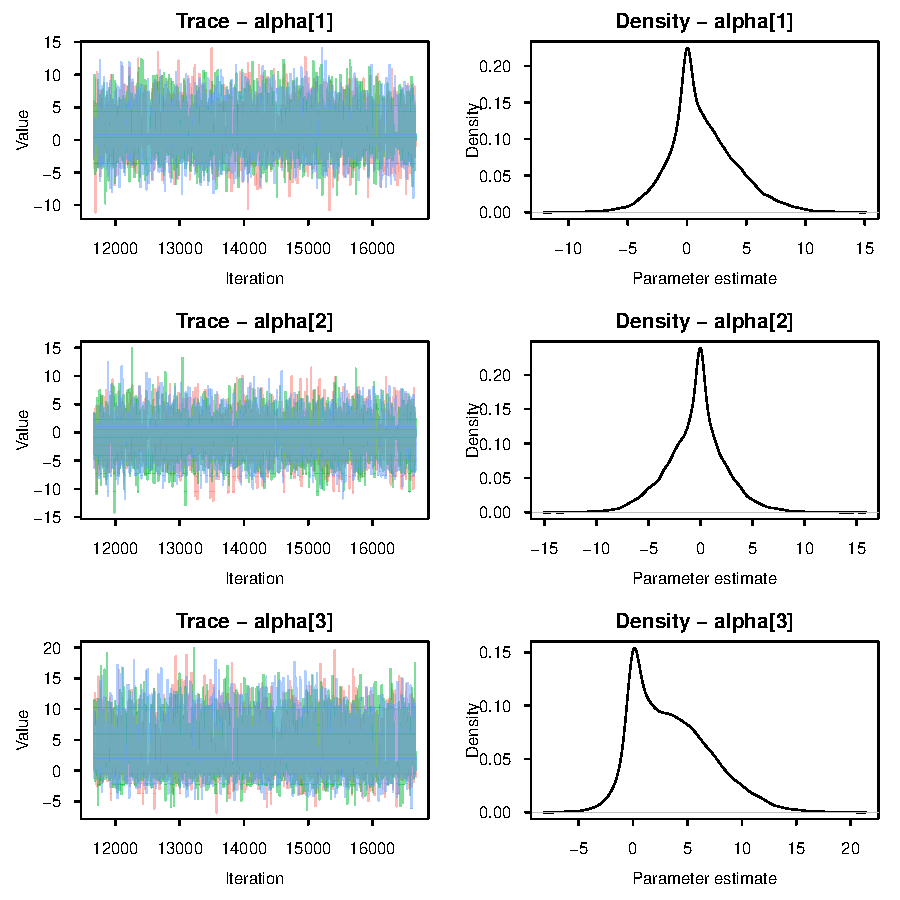
\includegraphics[width=.6\linewidth]{figure/FinalRFile-4350-Rnwauto-report-2} 

}




{\centering 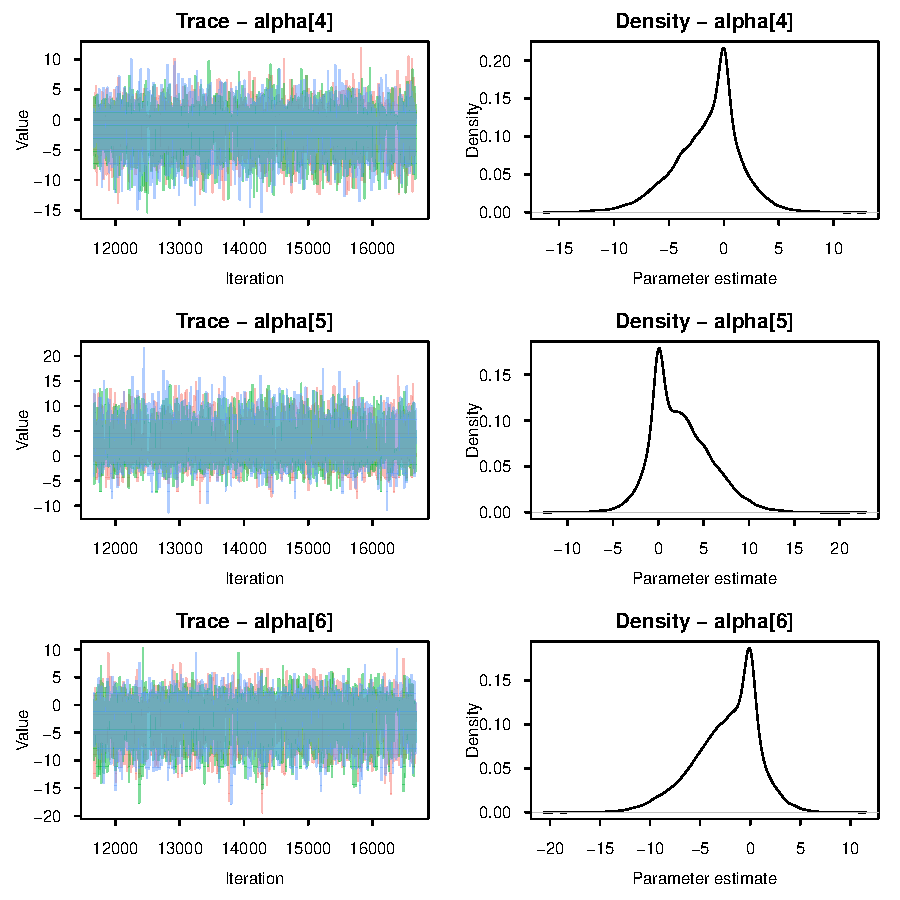
\includegraphics[width=.6\linewidth]{figure/FinalRFile-4350-Rnwauto-report-3} 

}




{\centering 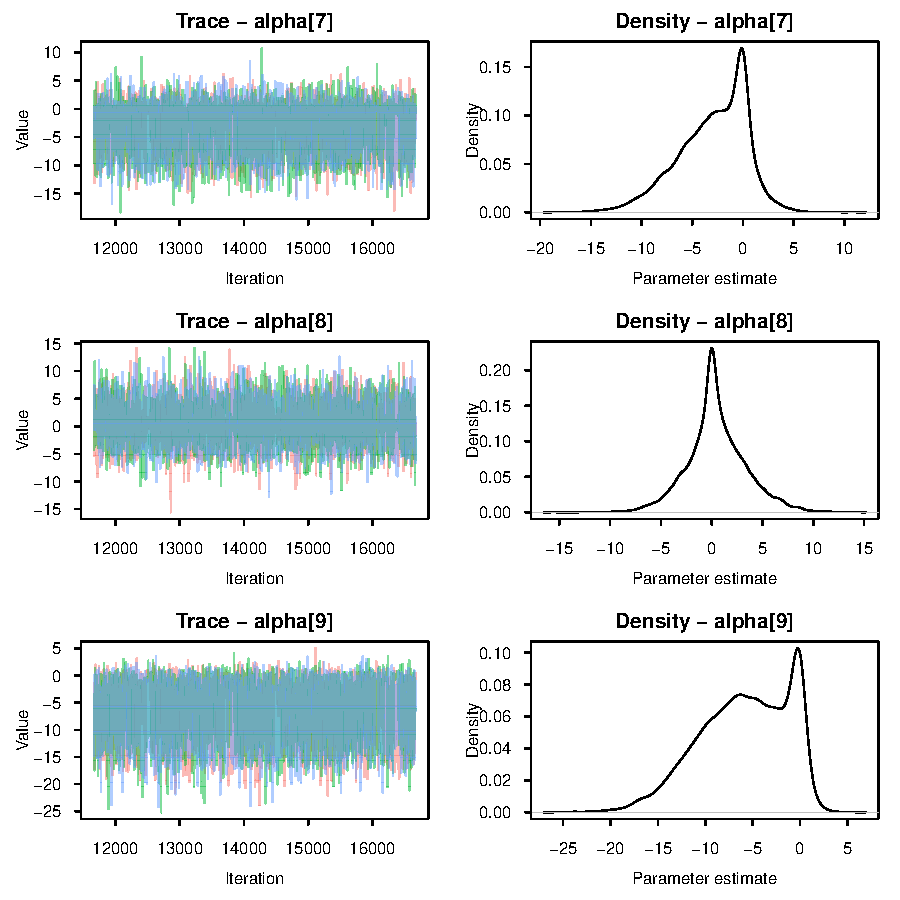
\includegraphics[width=.6\linewidth]{figure/FinalRFile-4350-Rnwauto-report-4} 

}




{\centering 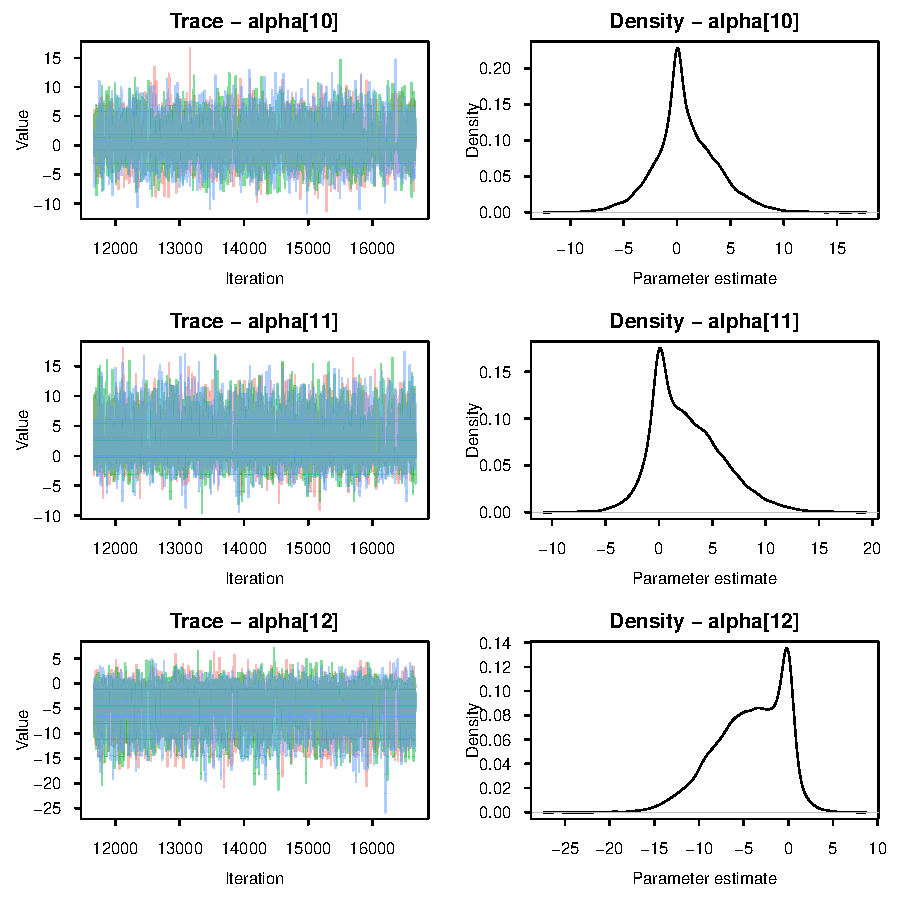
\includegraphics[width=.6\linewidth]{figure/FinalRFile-4350-Rnwauto-report-5} 

}




{\centering 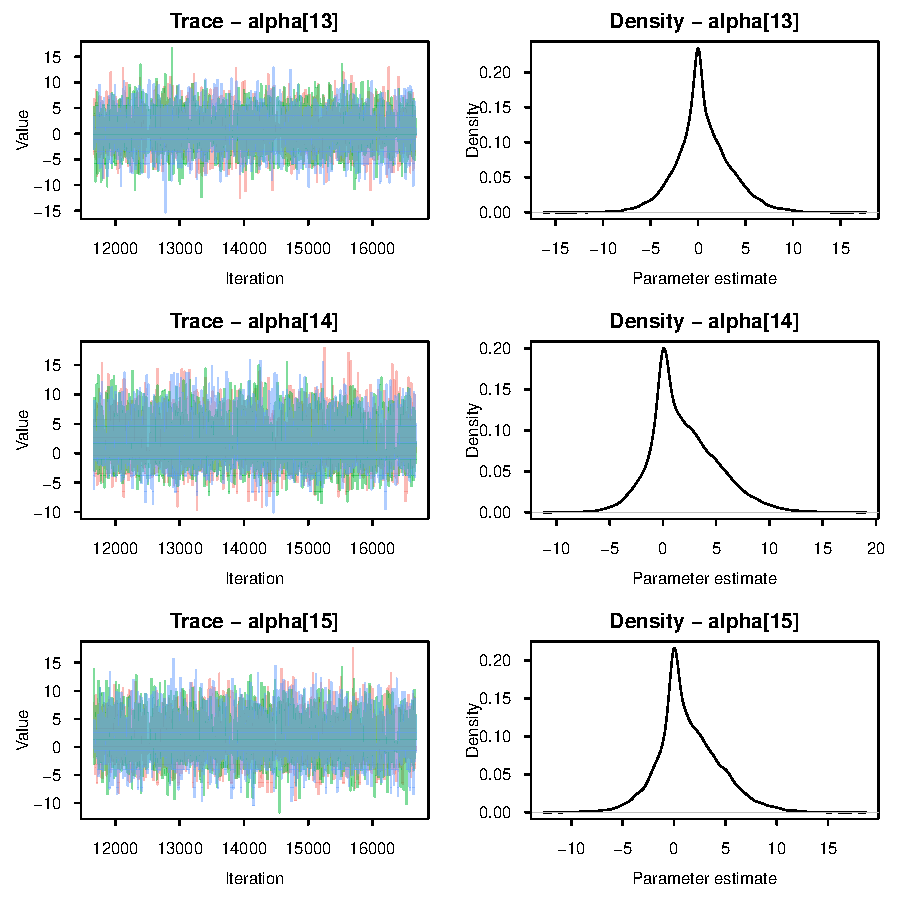
\includegraphics[width=.6\linewidth]{figure/FinalRFile-4350-Rnwauto-report-6} 

}




{\centering 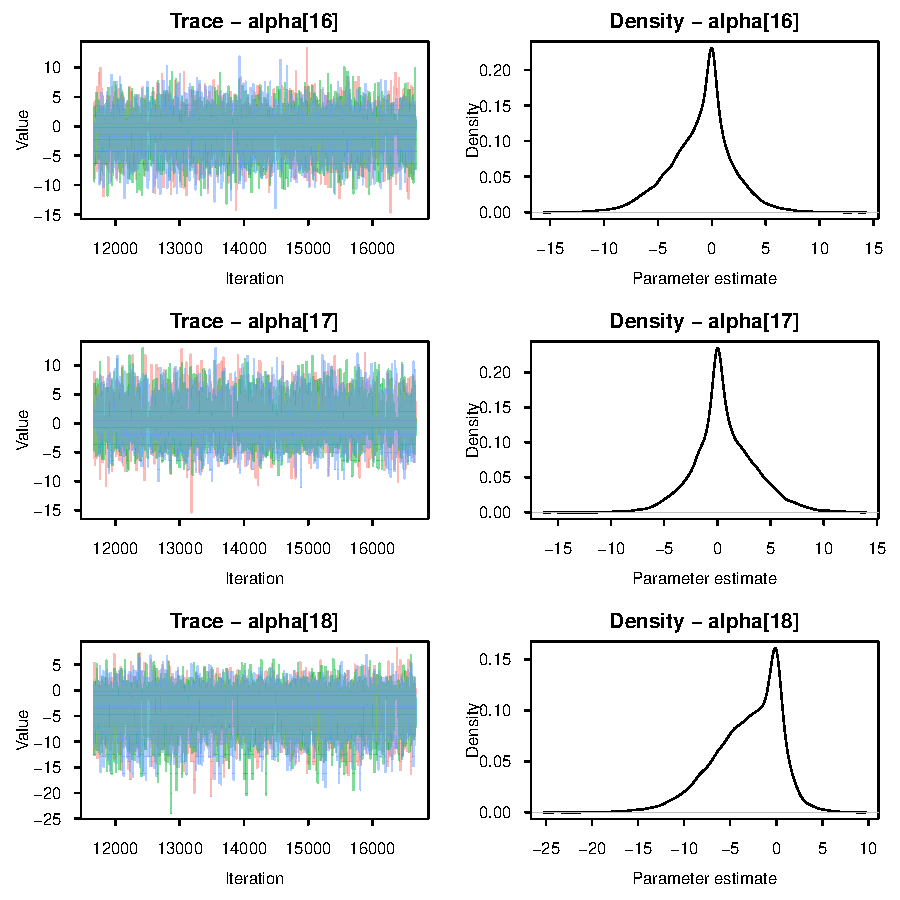
\includegraphics[width=.6\linewidth]{figure/FinalRFile-4350-Rnwauto-report-7} 

}




{\centering 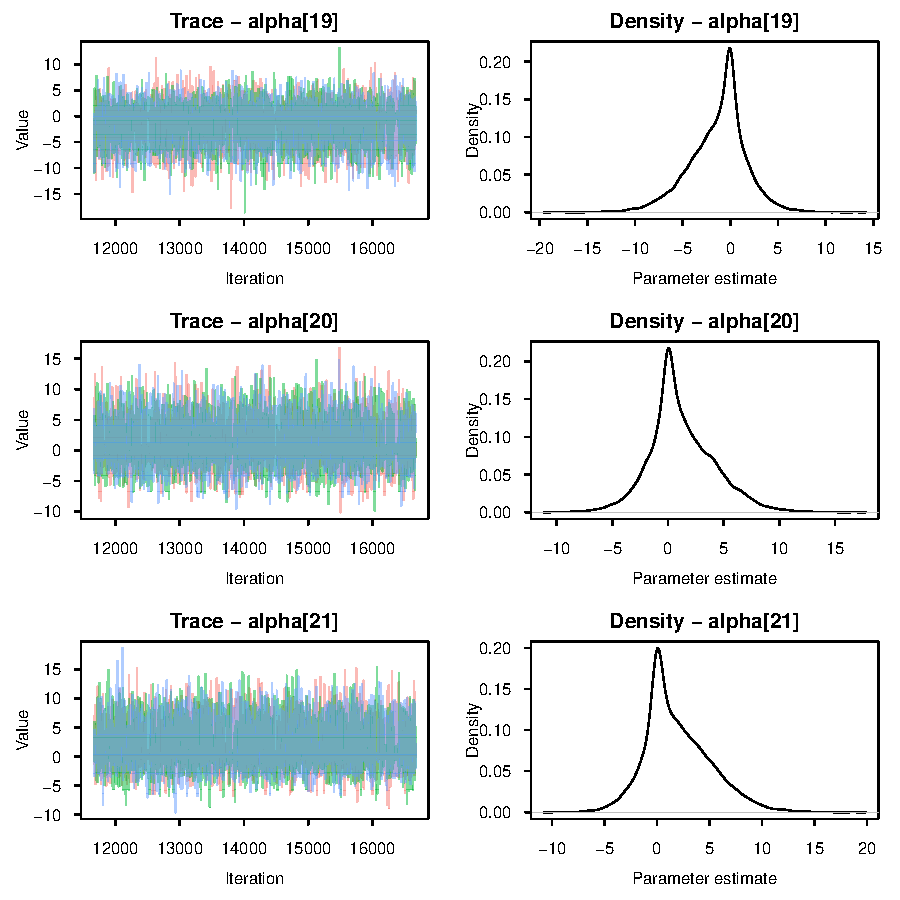
\includegraphics[width=.6\linewidth]{figure/FinalRFile-4350-Rnwauto-report-8} 

}




{\centering 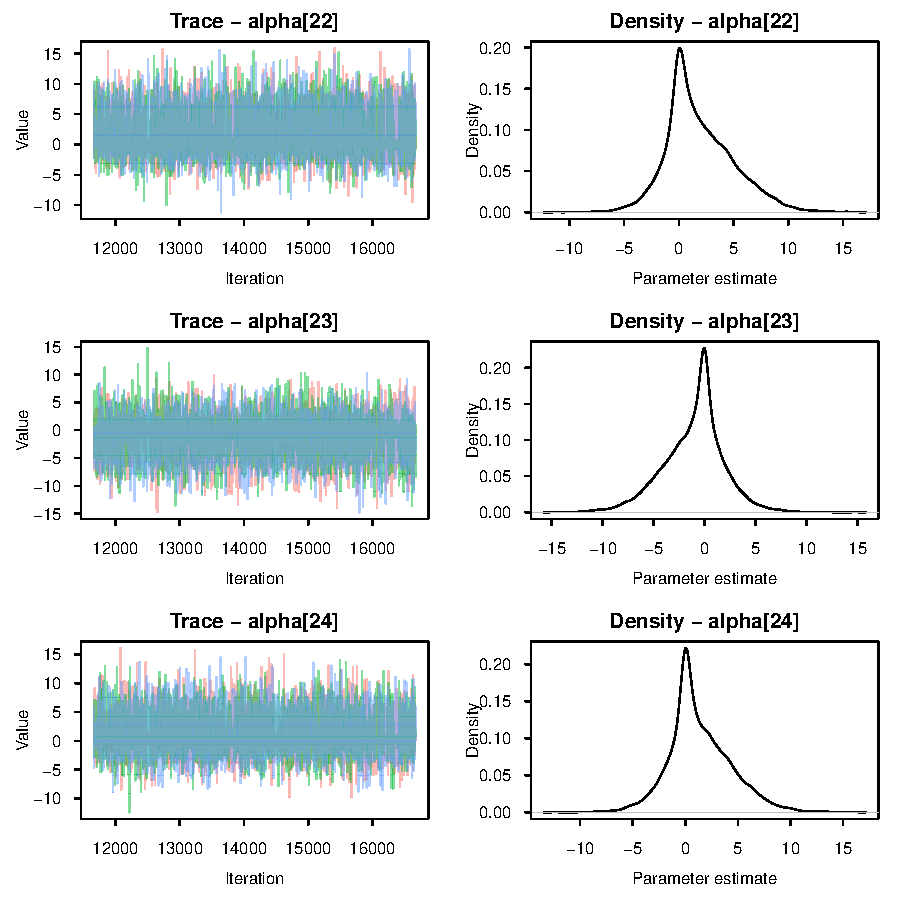
\includegraphics[width=.6\linewidth]{figure/FinalRFile-4350-Rnwauto-report-9} 

}




{\centering 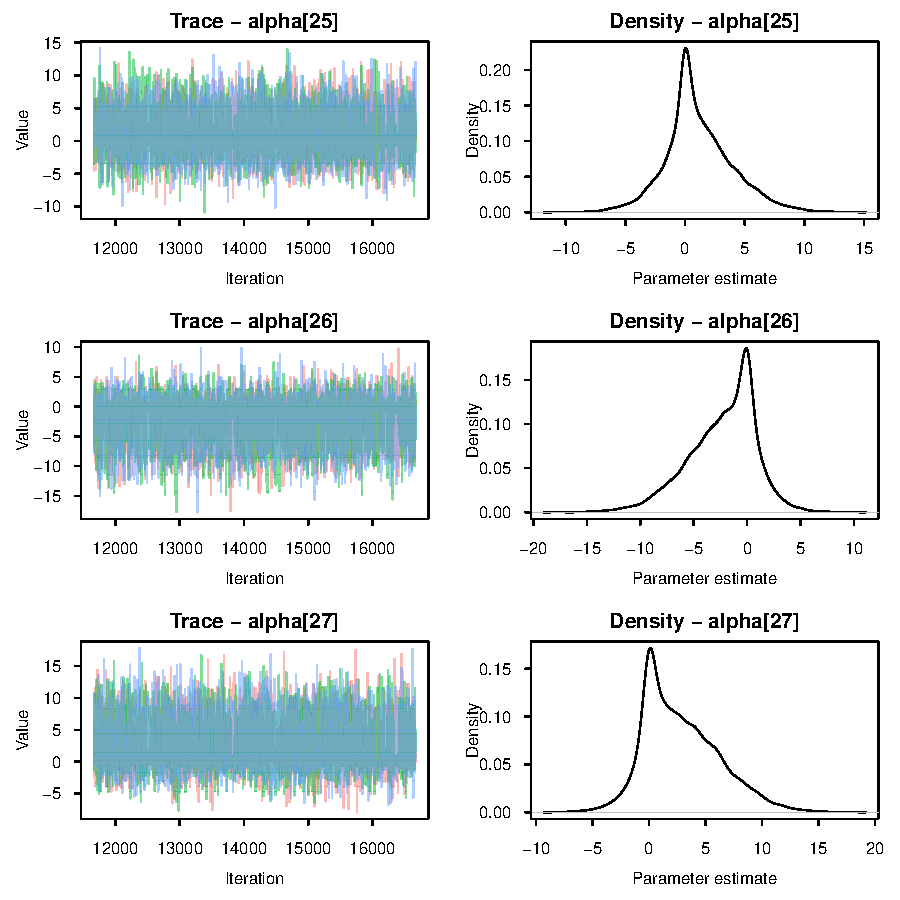
\includegraphics[width=.6\linewidth]{figure/FinalRFile-4350-Rnwauto-report-10} 

}




{\centering 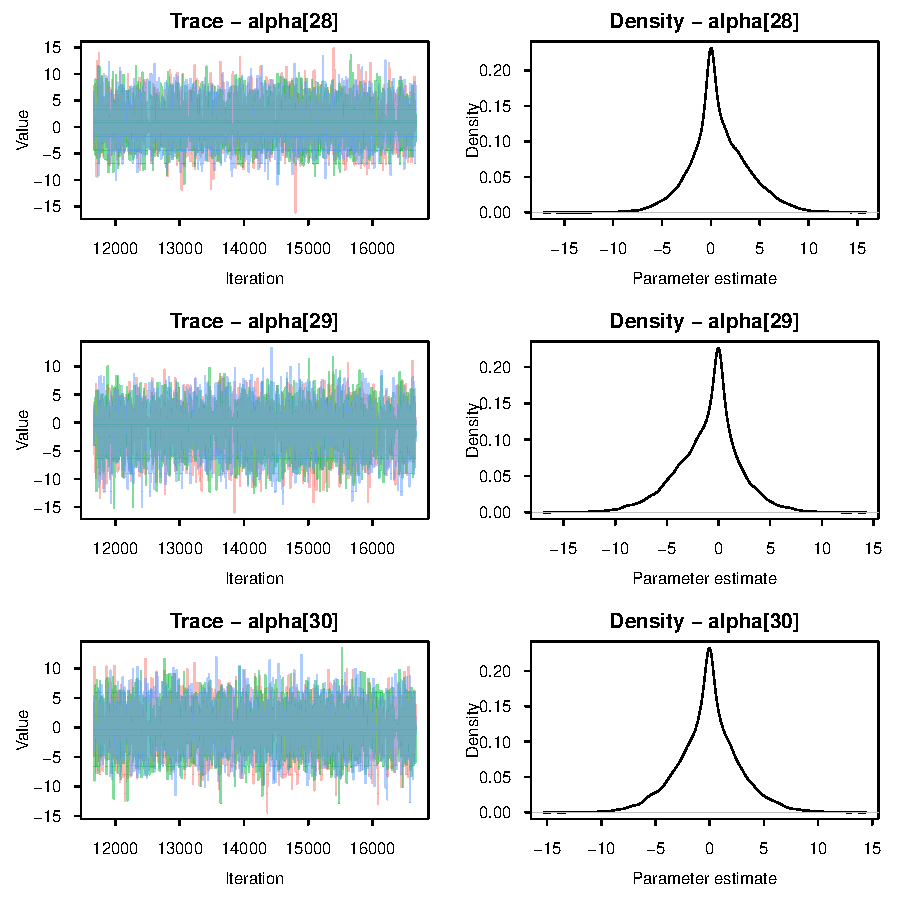
\includegraphics[width=.6\linewidth]{figure/FinalRFile-4350-Rnwauto-report-11} 

}




{\centering 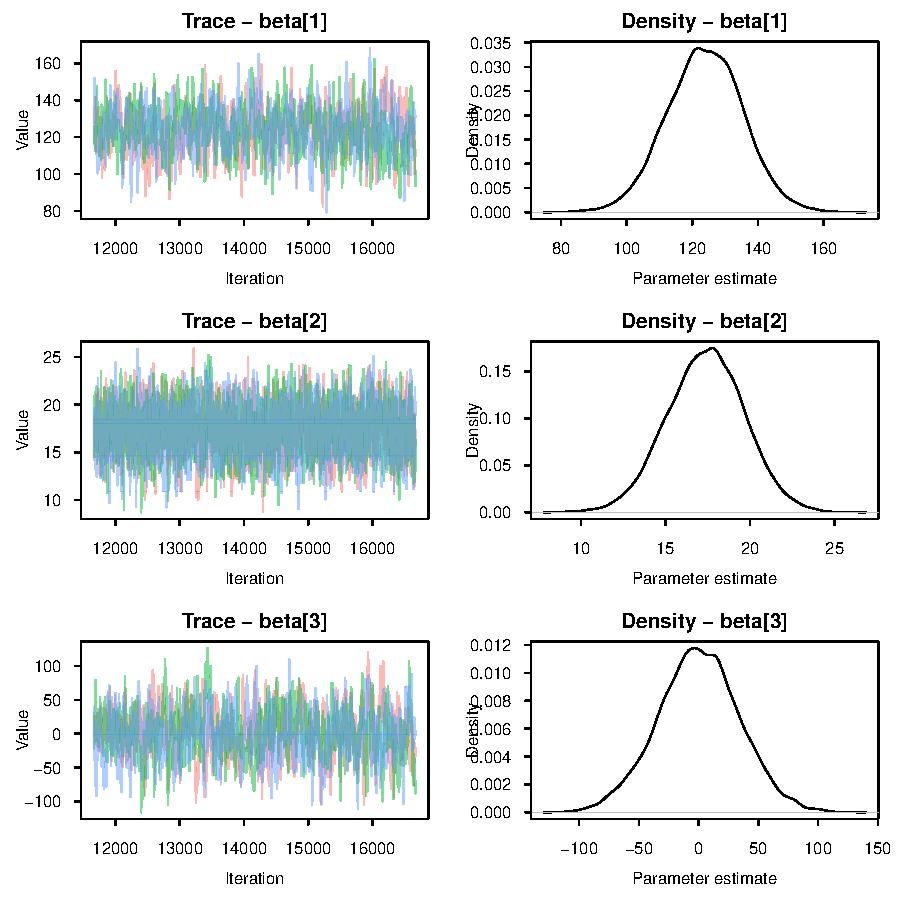
\includegraphics[width=.6\linewidth]{figure/FinalRFile-4350-Rnwauto-report-12} 

}




{\centering 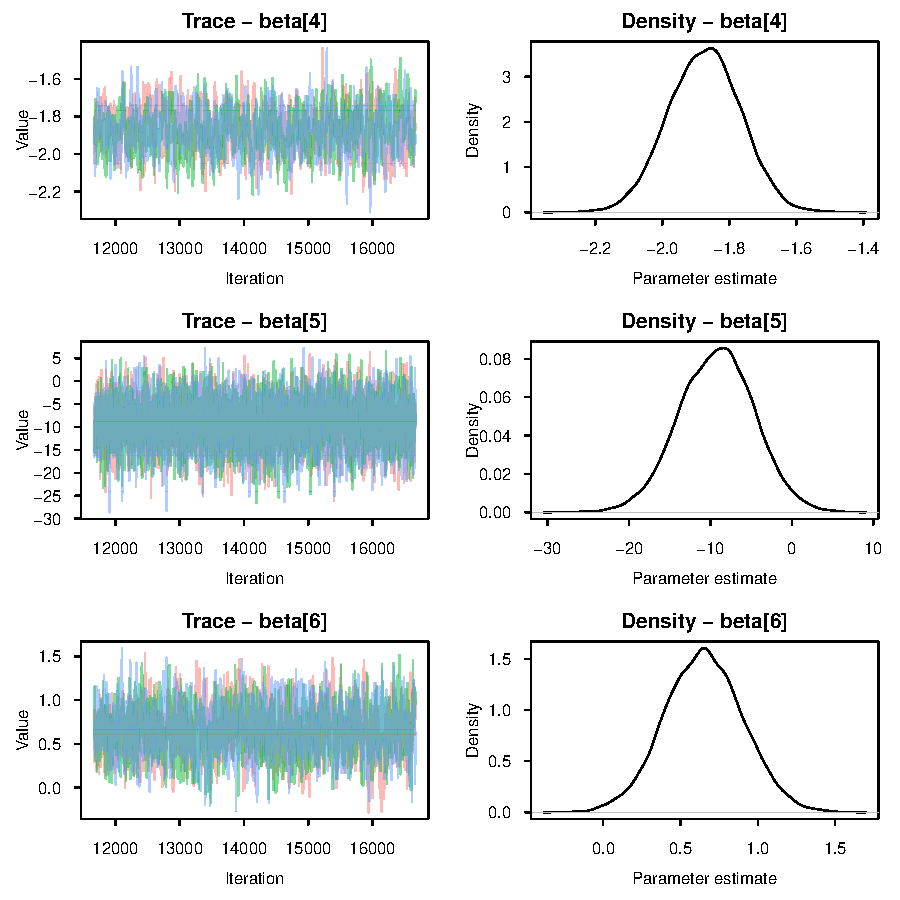
\includegraphics[width=.6\linewidth]{figure/FinalRFile-4350-Rnwauto-report-13} 

}




{\centering 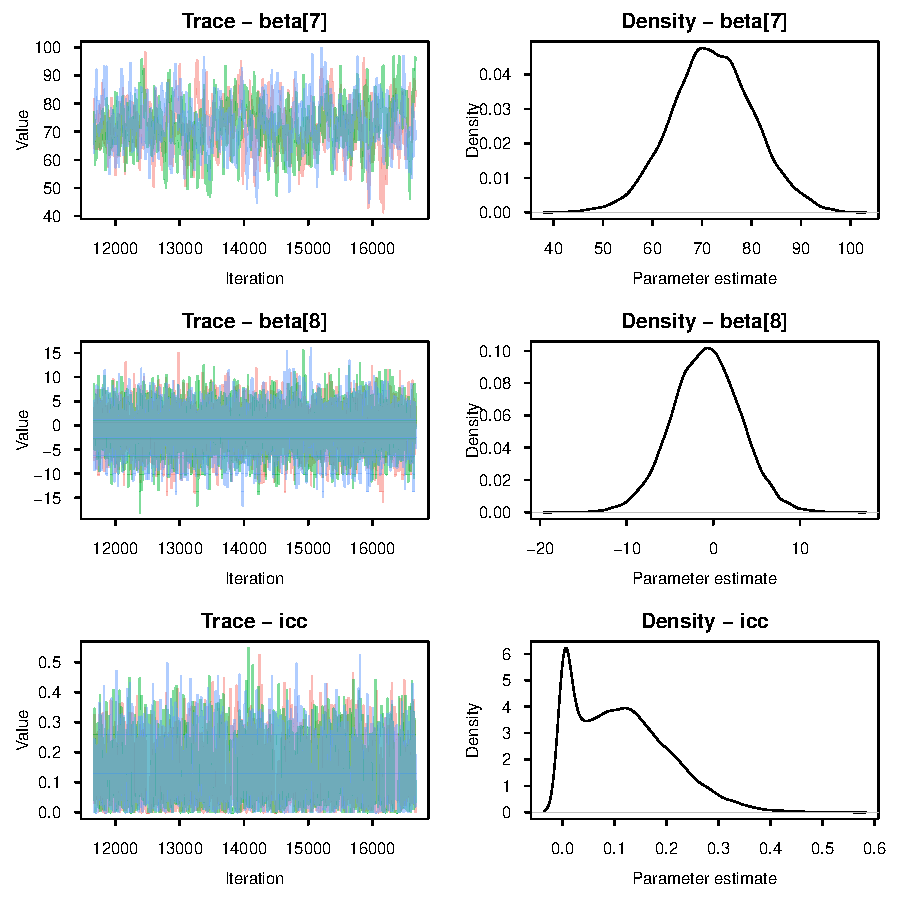
\includegraphics[width=.6\linewidth]{figure/FinalRFile-4350-Rnwauto-report-14} 

}




{\centering 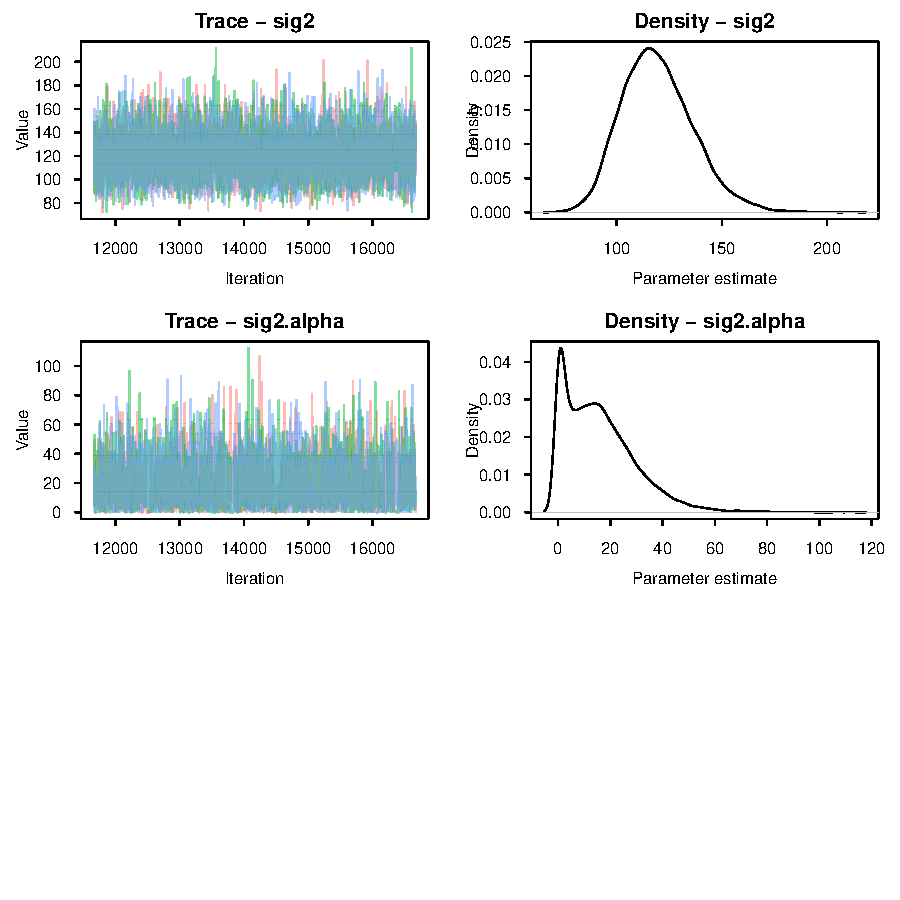
\includegraphics[width=.6\linewidth]{figure/FinalRFile-4350-Rnwauto-report-15} 

}


\begin{kframe}\begin{alltt}
\hlcom{# Examine the posterior distribution of the team random effect}
\hlstd{alphaSamples} \hlkwb{<-} \hlkwd{matrix}\hlstd{(}\hlnum{NA}\hlstd{,} \hlkwd{dim}\hlstd{(mcmcChain)[}\hlnum{1}\hlstd{], n.teams)}
\hlkwa{for}\hlstd{(i} \hlkwa{in} \hlnum{1}\hlopt{:}\hlstd{n.teams)\{}
  \hlstd{alphaSamples[,i]}  \hlkwb{<-} \hlstd{mcmcChain[,} \hlkwd{paste}\hlstd{(}\hlstr{"alpha["}\hlstd{,i,}\hlstr{"]"}\hlstd{,} \hlkwc{sep}\hlstd{=}\hlstr{""}\hlstd{)]}
\hlstd{\}}
\hlkwd{levels}\hlstd{(team_list)}
\end{alltt}
\begin{verbatim}
##  [1] "ARI" "ATL" "BAL" "BOS" "CHC" "CHW" "CIN" "CLE" "COL" "DET" "HOU" "KCR" "LAA" "LAD"
## [15] "MIA" "MIL" "MIN" "NYM" "NYY" "OAK" "PHI" "PIT" "SDP" "SEA" "SFG" "STL" "TBR" "TEX"
## [29] "TOR" "WSN"
\end{verbatim}
\begin{alltt}
\hlkwd{par}\hlstd{(}\hlkwc{mfrow}\hlstd{=}\hlkwd{c}\hlstd{(}\hlnum{1}\hlstd{,}\hlnum{1}\hlstd{),} \hlkwc{ask}\hlstd{=F)}
\hlkwd{boxplot}\hlstd{(}\hlkwd{as.data.frame}\hlstd{(alphaSamples),}
        \hlkwc{names}\hlstd{=}\hlkwd{as.character}\hlstd{(}\hlnum{1}\hlopt{:}\hlstd{n.teams),}
        \hlkwc{main}\hlstd{=}\hlstr{"Posterior samples of alphas"}\hlstd{,}
        \hlkwc{xlab}\hlstd{=}\hlstr{"Team"}\hlstd{)}
\hlkwd{abline}\hlstd{(}\hlkwc{h}\hlstd{=}\hlnum{0}\hlstd{)}
\end{alltt}
\end{kframe}

{\centering 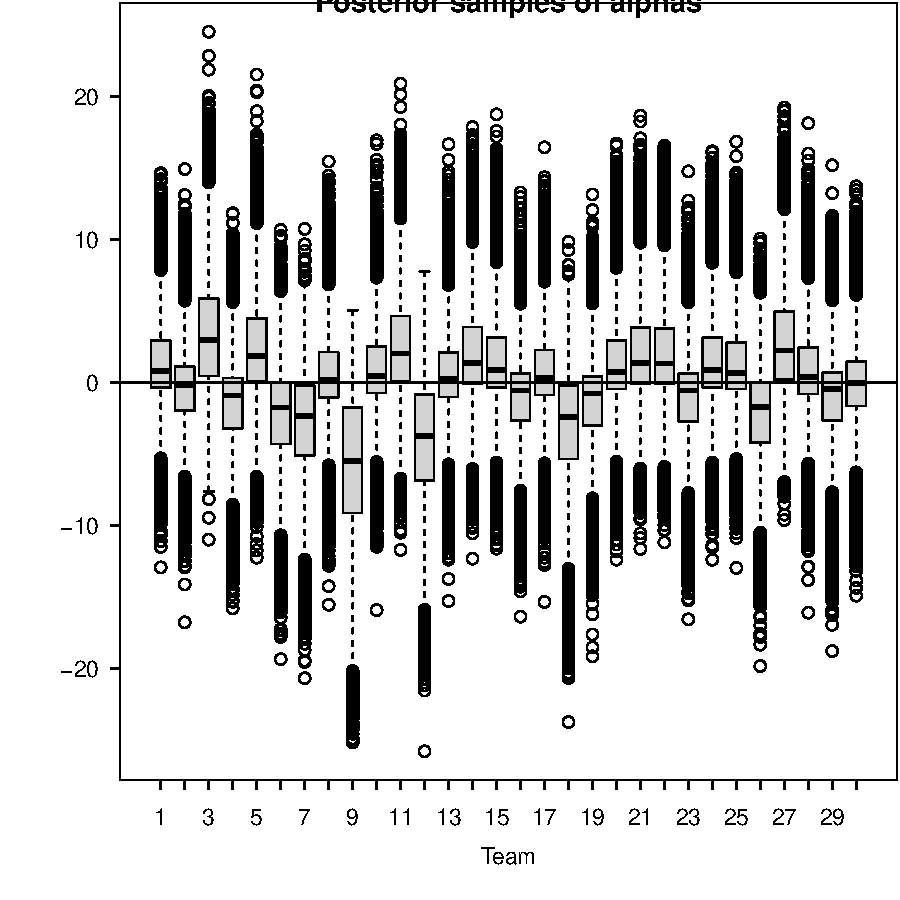
\includegraphics[width=.6\linewidth]{figure/FinalRFile-4350-Rnwauto-report-16} 

}


\begin{kframe}\begin{alltt}
\hlstd{teams_df} \hlkwb{=} \hlkwd{as.matrix}\hlstd{(}\hlkwd{data.frame}\hlstd{(}\hlkwc{num} \hlstd{=} \hlkwd{c}\hlstd{(}\hlnum{1}\hlopt{:}\hlnum{30}\hlstd{),}\hlkwc{team} \hlstd{=} \hlkwd{sort}\hlstd{(}\hlkwd{unique}\hlstd{(Team))))}

\hlstd{rank.alpha} \hlkwb{<-} \hlkwd{matrix}\hlstd{(}\hlnum{NA}\hlstd{,} \hlkwd{dim}\hlstd{(mcmcChain)[}\hlnum{1}\hlstd{], n.teams)}
\hlkwa{for}\hlstd{(i} \hlkwa{in} \hlnum{1}\hlopt{:}\hlkwd{dim}\hlstd{(mcmcChain)[}\hlnum{1}\hlstd{])\{}
  \hlstd{rank.alpha[i,]} \hlkwb{<-} \hlkwd{rank}\hlstd{(alphaSamples[i,])}
\hlstd{\}}
\hlstd{avg.rank} \hlkwb{<-} \hlkwd{rank}\hlstd{(}\hlkwd{apply}\hlstd{(rank.alpha,} \hlnum{2}\hlstd{, mean))}


\hlcom{# par(mfrow=c(1,1), ask=F)}
\hlcom{# plot(c(-15,15), c(1,30), type='n', axes=F, xlab="", ylab="", main="Team Rankings")}
\hlcom{# axis(1,at=seq(-20, 20, length=5))}
\hlcom{# for(i in 1:n.teams)\{}
\hlcom{#   lines(quantile(alphaSamples[,i], c(0.025,0.975)), rep(avg.rank[i],2))}
\hlcom{#   points(mean(alphaSamples[,i]), avg.rank[i], pch=19)}
\hlcom{#   text(15, avg.rank[i], i, cex=.5)}
\hlcom{# \}}

\hlcom{# ranked_teams = vector()}
\hlcom{# }
\hlcom{# }
\hlcom{# for(i in 1:n.teams)\{}
\hlcom{#   for(j in 1:n.teams)\{}
\hlcom{#     if (avg.rank[j] == i)\{}
\hlcom{#       ranked_teams[i]<- teams_df[j,2]}
\hlcom{#     \}}
\hlcom{#   \}}
\hlcom{# \}}
\hlcom{# ranked_teams}

\hlstd{ranked_teams_idx} \hlkwb{=} \hlkwd{vector}\hlstd{()}
\hlkwa{for}\hlstd{(i} \hlkwa{in} \hlnum{1}\hlopt{:}\hlstd{n.teams)\{}
  \hlkwa{for}\hlstd{(j} \hlkwa{in} \hlnum{1}\hlopt{:}\hlstd{n.teams)\{}
    \hlkwa{if} \hlstd{(avg.rank[j]} \hlopt{==} \hlstd{i)\{}
      \hlstd{ranked_teams_idx[i]}\hlkwb{<-} \hlstd{teams_df[j,}\hlnum{1}\hlstd{]}
    \hlstd{\}}
  \hlstd{\}}
\hlstd{\}}
\hlstd{ranked_teams_idx} \hlkwb{=} \hlkwd{trimws}\hlstd{(ranked_teams_idx)}

\hlcom{# Sorted Alphas}
\hlstd{temp_vec}\hlkwb{=}\hlkwd{vector}\hlstd{()}
\hlkwa{for}\hlstd{(i} \hlkwa{in} \hlnum{1}\hlopt{:}\hlstd{n.teams)\{}
  \hlstd{temp_vec[i]} \hlkwb{=} \hlkwd{paste0}\hlstd{(}\hlstr{'alpha['}\hlstd{,ranked_teams_idx[i],}\hlstr{']'}\hlstd{)}
\hlstd{\}}

\hlkwd{library}\hlstd{(bayesplot)}

\hlcom{# Plot the alphas to see random effects}
\hlkwd{mcmc_intervals}\hlstd{(codaSamples,}\hlkwc{regex_pars} \hlstd{=} \hlstr{'^[alpha]'}\hlstd{)}\hlopt{+}
  \hlkwd{scale_y_discrete}\hlstd{(}
    \hlkwc{labels} \hlstd{=}
      \hlkwd{c}\hlstd{(}\hlstr{'alpha[1]'} \hlstd{=} \hlkwd{levels}\hlstd{(team_list)[}\hlnum{1}\hlstd{],}
        \hlstr{'alpha[2]'} \hlstd{=} \hlkwd{levels}\hlstd{(team_list)[}\hlnum{2}\hlstd{],}
        \hlstr{'alpha[3]'} \hlstd{=} \hlkwd{levels}\hlstd{(team_list)[}\hlnum{3}\hlstd{],}
        \hlstr{'alpha[4]'} \hlstd{=} \hlkwd{levels}\hlstd{(team_list)[}\hlnum{4}\hlstd{],}
        \hlstr{'alpha[5]'} \hlstd{=} \hlkwd{levels}\hlstd{(team_list)[}\hlnum{5}\hlstd{],}
        \hlstr{'alpha[6]'} \hlstd{=} \hlkwd{levels}\hlstd{(team_list)[}\hlnum{6}\hlstd{],}
        \hlstr{'alpha[7]'} \hlstd{=} \hlkwd{levels}\hlstd{(team_list)[}\hlnum{7}\hlstd{],}
        \hlstr{'alpha[8]'} \hlstd{=} \hlkwd{levels}\hlstd{(team_list)[}\hlnum{8}\hlstd{],}
        \hlstr{'alpha[9]'} \hlstd{=} \hlkwd{levels}\hlstd{(team_list)[}\hlnum{9}\hlstd{],}
        \hlstr{'alpha[10]'} \hlstd{=} \hlkwd{levels}\hlstd{(team_list)[}\hlnum{10}\hlstd{],}
        \hlstr{'alpha[11]'} \hlstd{=} \hlkwd{levels}\hlstd{(team_list)[}\hlnum{11}\hlstd{],}
        \hlstr{'alpha[12]'} \hlstd{=} \hlkwd{levels}\hlstd{(team_list)[}\hlnum{12}\hlstd{],}
        \hlstr{'alpha[13]'} \hlstd{=} \hlkwd{levels}\hlstd{(team_list)[}\hlnum{13}\hlstd{],}
        \hlstr{'alpha[14]'} \hlstd{=} \hlkwd{levels}\hlstd{(team_list)[}\hlnum{14}\hlstd{],}
        \hlstr{'alpha[15]'} \hlstd{=} \hlkwd{levels}\hlstd{(team_list)[}\hlnum{15}\hlstd{],}
        \hlstr{'alpha[16]'} \hlstd{=} \hlkwd{levels}\hlstd{(team_list)[}\hlnum{16}\hlstd{],}
        \hlstr{'alpha[17]'} \hlstd{=} \hlkwd{levels}\hlstd{(team_list)[}\hlnum{17}\hlstd{],}
        \hlstr{'alpha[18]'} \hlstd{=} \hlkwd{levels}\hlstd{(team_list)[}\hlnum{18}\hlstd{],}
        \hlstr{'alpha[19]'} \hlstd{=} \hlkwd{levels}\hlstd{(team_list)[}\hlnum{19}\hlstd{],}
        \hlstr{'alpha[20]'} \hlstd{=} \hlkwd{levels}\hlstd{(team_list)[}\hlnum{20}\hlstd{],}
        \hlstr{'alpha[21]'} \hlstd{=} \hlkwd{levels}\hlstd{(team_list)[}\hlnum{21}\hlstd{],}
        \hlstr{'alpha[22]'} \hlstd{=} \hlkwd{levels}\hlstd{(team_list)[}\hlnum{22}\hlstd{],}
        \hlstr{'alpha[23]'} \hlstd{=} \hlkwd{levels}\hlstd{(team_list)[}\hlnum{23}\hlstd{],}
        \hlstr{'alpha[24]'} \hlstd{=} \hlkwd{levels}\hlstd{(team_list)[}\hlnum{24}\hlstd{],}
        \hlstr{'alpha[25]'} \hlstd{=} \hlkwd{levels}\hlstd{(team_list)[}\hlnum{25}\hlstd{],}
        \hlstr{'alpha[26]'} \hlstd{=} \hlkwd{levels}\hlstd{(team_list)[}\hlnum{26}\hlstd{],}
        \hlstr{'alpha[27]'} \hlstd{=} \hlkwd{levels}\hlstd{(team_list)[}\hlnum{27}\hlstd{],}
        \hlstr{'alpha[28]'} \hlstd{=} \hlkwd{levels}\hlstd{(team_list)[}\hlnum{28}\hlstd{],}
        \hlstr{'alpha[29]'} \hlstd{=} \hlkwd{levels}\hlstd{(team_list)[}\hlnum{29}\hlstd{],}
        \hlstr{'alpha[30]'} \hlstd{=} \hlkwd{levels}\hlstd{(team_list)[}\hlnum{30}\hlstd{]),}
    \hlkwc{limits} \hlstd{=} \hlkwd{c}\hlstd{(temp_vec)}
  \hlstd{)}\hlopt{+}
  \hlkwd{ggtitle}\hlstd{(}\hlstr{'MLB teams random effects'}\hlstd{)}\hlopt{+}
  \hlkwd{theme}\hlstd{(}\hlkwc{plot.title} \hlstd{=} \hlkwd{element_text}\hlstd{(}\hlkwc{hjust} \hlstd{=} \hlnum{0.5}\hlstd{))}
\end{alltt}


{\ttfamily\noindent\itshape\color{messagecolor}{\#\# Scale for 'y' is already present. Adding another scale for 'y', which will replace the\\\#\# existing scale.}}\end{kframe}

{\centering 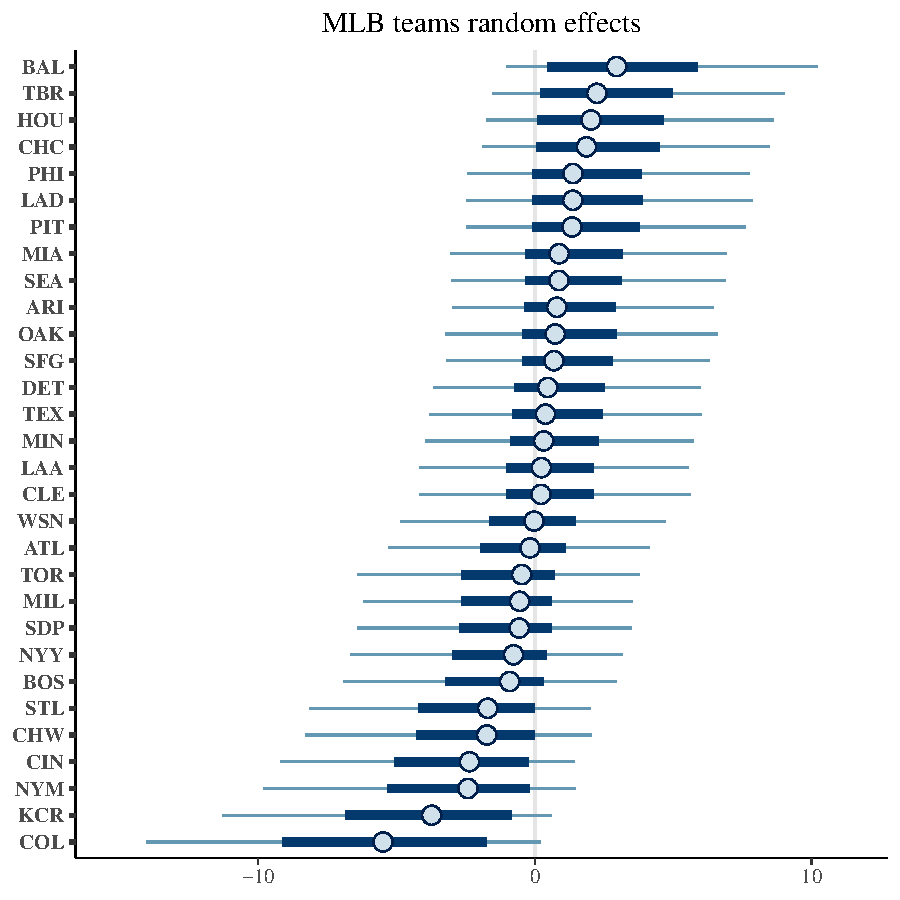
\includegraphics[width=.6\linewidth]{figure/FinalRFile-4350-Rnwauto-report-17} 

}


\begin{kframe}\begin{alltt}
\hlstd{era.xera} \hlkwb{=} \hlkwd{read.csv}\hlstd{(}\hlstr{'era_vs_expected.csv'}\hlstd{)}
\hlstd{era.xera} \hlkwb{=} \hlstd{era.xera[}\hlkwd{order}\hlstd{(era.xera}\hlopt{$}\hlstd{diff),]}
\hlstd{era.xera}\hlopt{$}\hlstd{Team} \hlkwb{<-} \hlkwd{factor}\hlstd{(era.xera}\hlopt{$}\hlstd{Team,} \hlkwc{levels} \hlstd{= era.xera}\hlopt{$}\hlstd{Team[}\hlkwd{order}\hlstd{(era.xera}\hlopt{$}\hlstd{diff)])}
\hlkwd{ggplot}\hlstd{(}\hlkwc{data} \hlstd{= era.xera,} \hlkwd{aes}\hlstd{(}\hlkwc{x} \hlstd{= Team,}\hlkwc{y}\hlstd{=diff))}\hlopt{+}
  \hlkwd{geom_bar}\hlstd{(}\hlkwc{stat}\hlstd{=}\hlstr{'identity'}\hlstd{)}\hlopt{+}
  \hlkwd{coord_flip}\hlstd{()}\hlopt{+}
  \hlkwd{ggtitle}\hlstd{(}\hlstr{'ERA - xERA from FanGraphs'}\hlstd{)}\hlopt{+}
  \hlkwd{theme}\hlstd{(}\hlkwc{plot.title} \hlstd{=} \hlkwd{element_text}\hlstd{(}\hlkwc{hjust} \hlstd{=} \hlnum{0.5}\hlstd{))}
\end{alltt}
\end{kframe}

{\centering 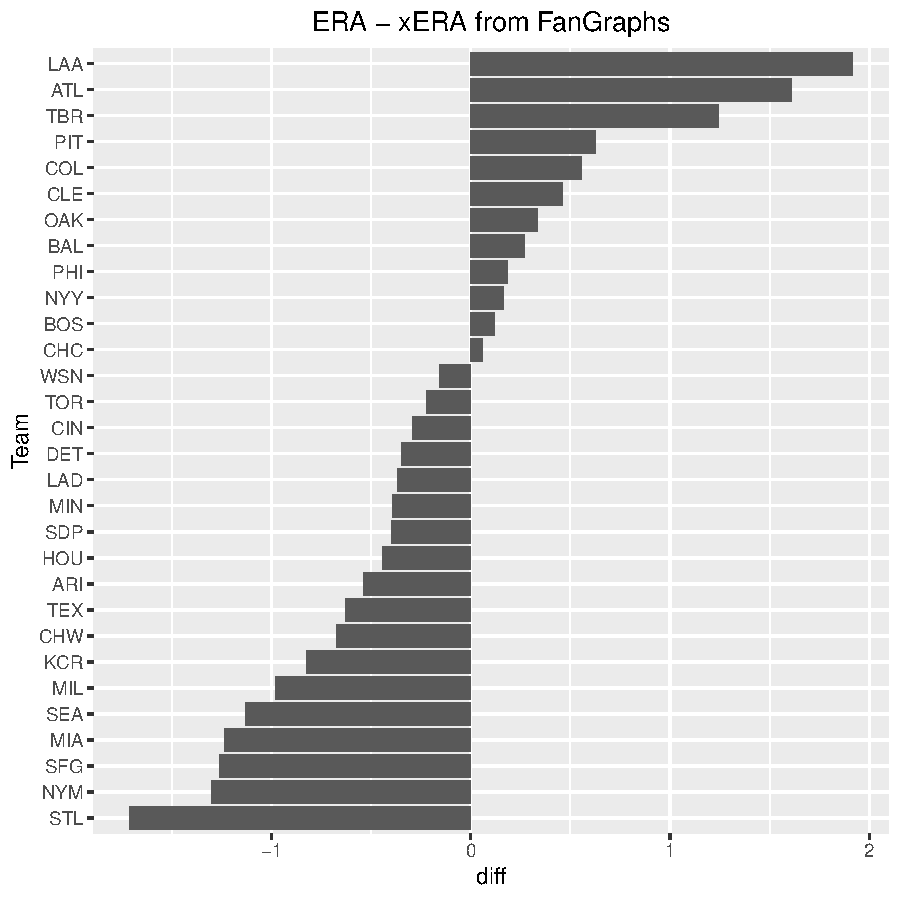
\includegraphics[width=.6\linewidth]{figure/FinalRFile-4350-Rnwauto-report-18} 

}


\begin{kframe}\begin{alltt}
\hlstd{fip.xfip} \hlkwb{=} \hlkwd{read.csv}\hlstd{(}\hlstr{'FIP_vs_xFIP.csv'}\hlstd{)}
\hlstd{fip.xfip} \hlkwb{=} \hlstd{fip.xfip[}\hlkwd{order}\hlstd{(fip.xfip}\hlopt{$}\hlstd{diff),]}
\hlstd{fip.xfip}\hlopt{$}\hlstd{Team} \hlkwb{<-} \hlkwd{factor}\hlstd{(fip.xfip}\hlopt{$}\hlstd{Team,} \hlkwc{levels} \hlstd{= fip.xfip}\hlopt{$}\hlstd{Team[}\hlkwd{order}\hlstd{(fip.xfip}\hlopt{$}\hlstd{diff)])}
\hlkwd{ggplot}\hlstd{(}\hlkwc{data} \hlstd{= fip.xfip,} \hlkwd{aes}\hlstd{(}\hlkwc{x} \hlstd{= Team,}\hlkwc{y}\hlstd{=diff))}\hlopt{+}
  \hlkwd{geom_bar}\hlstd{(}\hlkwc{stat}\hlstd{=}\hlstr{'identity'}\hlstd{)}\hlopt{+}
  \hlkwd{coord_flip}\hlstd{()}\hlopt{+}
  \hlkwd{ggtitle}\hlstd{(}\hlstr{'FIP-  -  xFIP- from FanGraphs'}\hlstd{)}\hlopt{+}
  \hlkwd{theme}\hlstd{(}\hlkwc{plot.title} \hlstd{=} \hlkwd{element_text}\hlstd{(}\hlkwc{hjust} \hlstd{=} \hlnum{0.5}\hlstd{))}
\end{alltt}
\end{kframe}

{\centering 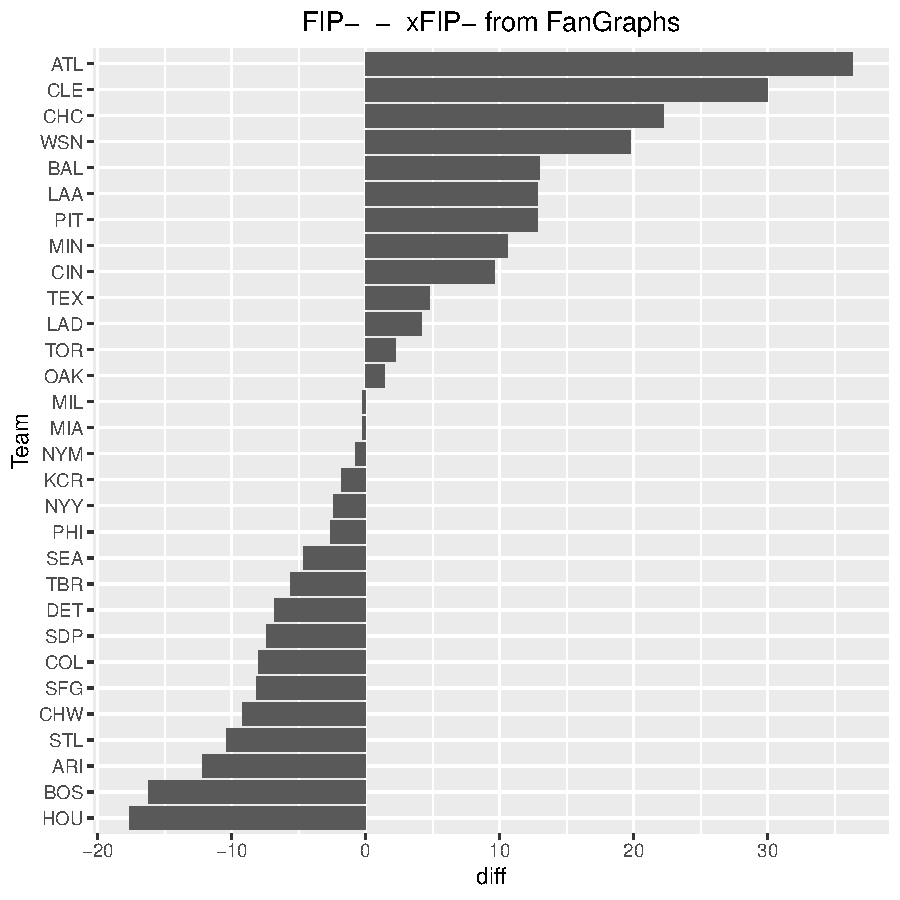
\includegraphics[width=.6\linewidth]{figure/FinalRFile-4350-Rnwauto-report-19} 

}


\begin{kframe}\begin{alltt}
\hlcom{# Boxplot of posteriors for beta}
\hlkwd{boxplot}\hlstd{(mcmcChain[,}\hlnum{31}\hlopt{:}\hlnum{38}\hlstd{],} \hlkwc{main} \hlstd{=} \hlstr{"Posterior samples of beta"}\hlstd{,}
        \hlkwc{names}\hlstd{=}\hlkwd{c}\hlstd{(}\hlstr{"Intercept"}\hlstd{,}
                \hlstr{"HR9"}\hlstd{,}
                \hlstr{"BABIP"}\hlstd{,}
                \hlstr{"LOB"}\hlstd{,}
                \hlstr{"WAR"}\hlstd{,}
                \hlstr{"KBB"}\hlstd{,}
                \hlstr{"WHIP"}\hlstd{,}
                \hlstr{"WIN"}\hlstd{))}
\hlkwd{abline}\hlstd{(}\hlkwc{h} \hlstd{=} \hlnum{0}\hlstd{,} \hlkwc{lty} \hlstd{=} \hlnum{2}\hlstd{,} \hlkwc{col}\hlstd{=}\hlstr{"red"}\hlstd{)}
\end{alltt}
\end{kframe}

{\centering 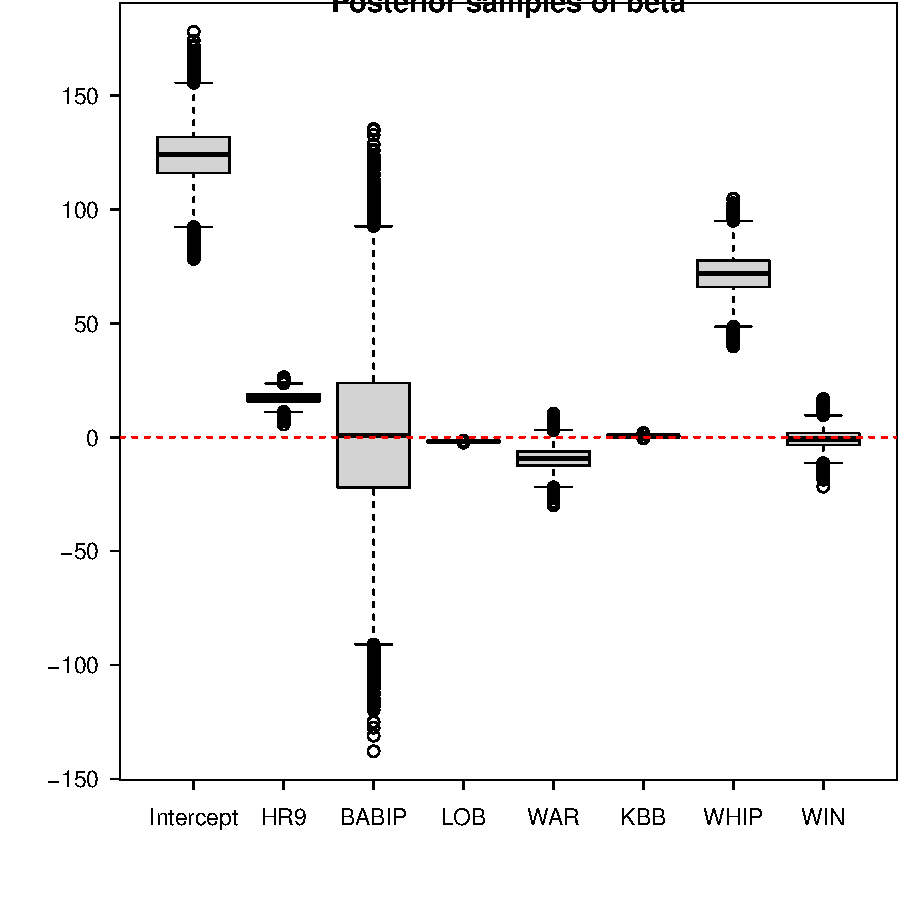
\includegraphics[width=.6\linewidth]{figure/FinalRFile-4350-Rnwauto-report-20} 

}


\begin{kframe}\begin{alltt}
\hlcom{# 50% (thin line) and 95% (thick line) credible interval "caterpillar" plots}
\hlcom{# dot is the posterior median}
\hlkwd{MCMCplot}\hlstd{(codaSamples,} \hlkwc{params} \hlstd{=} \hlstr{"beta"}\hlstd{,}
         \hlkwc{main} \hlstd{=} \hlstr{"Posterior CIs for beta"}\hlstd{)}
\end{alltt}
\end{kframe}

{\centering 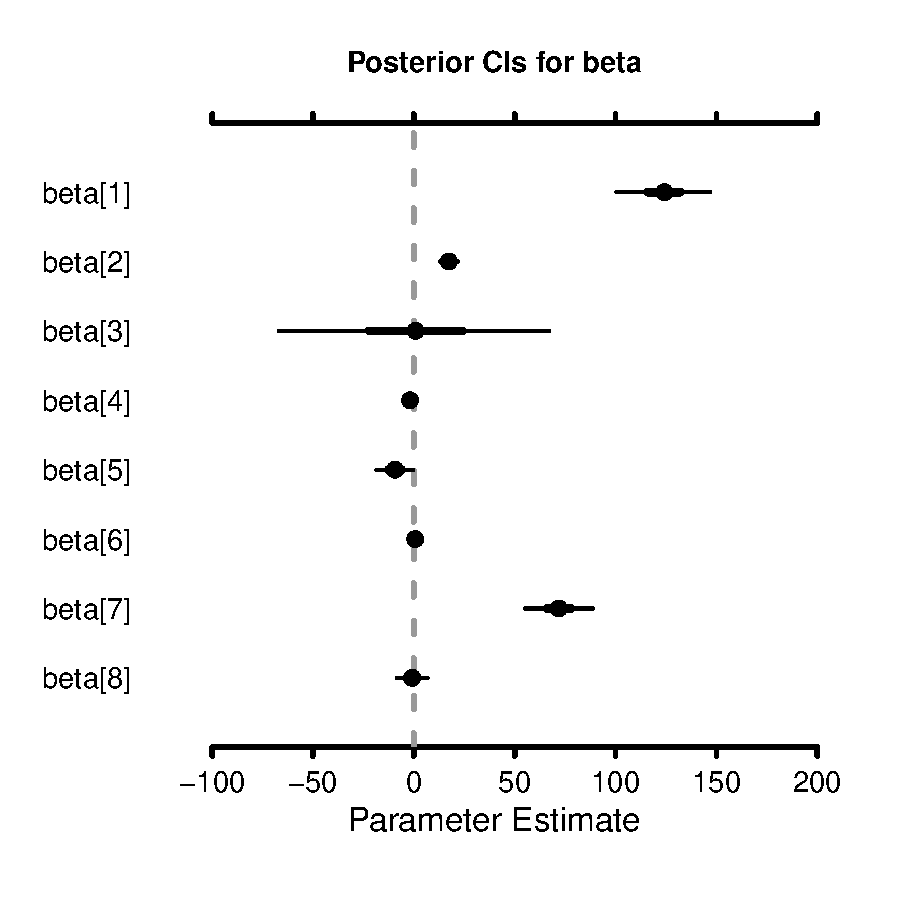
\includegraphics[width=.6\linewidth]{figure/FinalRFile-4350-Rnwauto-report-21} 

}


\begin{kframe}\begin{alltt}
\hlkwd{MCMCplot}\hlstd{(codaSamples,} \hlkwc{params} \hlstd{=} \hlkwd{c}\hlstd{(}\hlstr{"sig2"}\hlstd{,}\hlstr{'sig2.alpha'}\hlstd{),}
         \hlkwc{main} \hlstd{=} \hlstr{"Posterior CIs for sigmas"}\hlstd{)}
\end{alltt}
\end{kframe}

{\centering 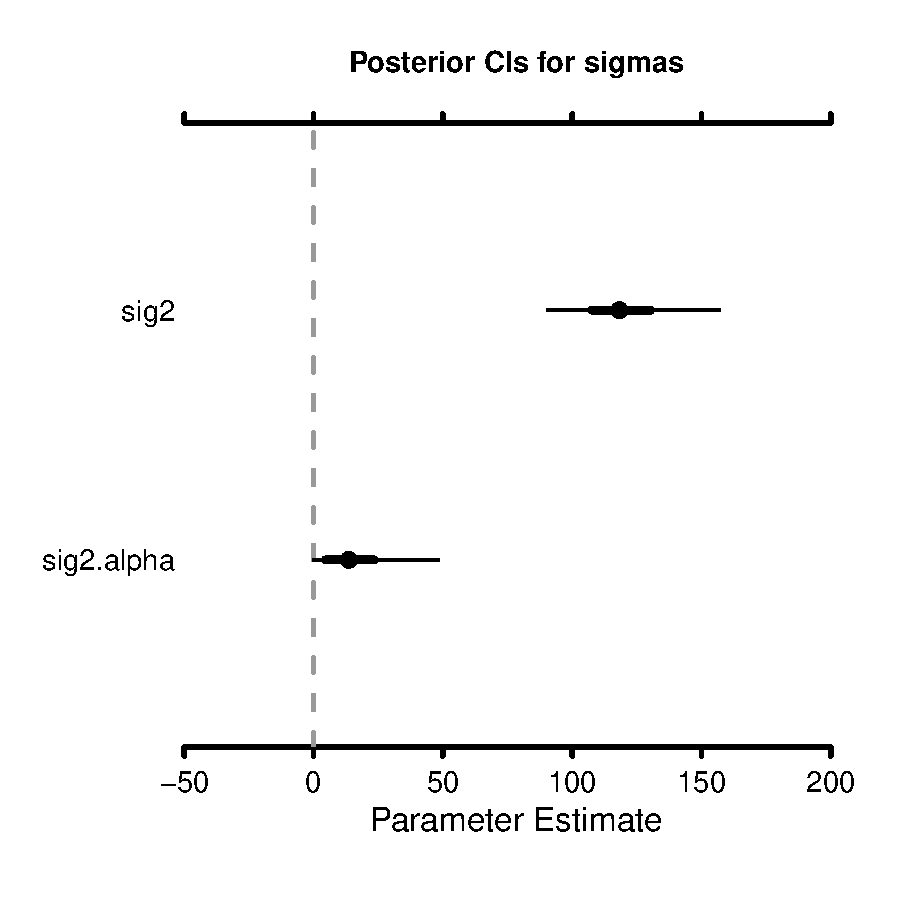
\includegraphics[width=.6\linewidth]{figure/FinalRFile-4350-Rnwauto-report-22} 

}


\begin{kframe}\begin{alltt}
\hlcom{# Posterior for intraclass correlation}
\hlkwd{plot}\hlstd{(codaSamples[,}\hlnum{39}\hlstd{])}
\end{alltt}
\end{kframe}

{\centering 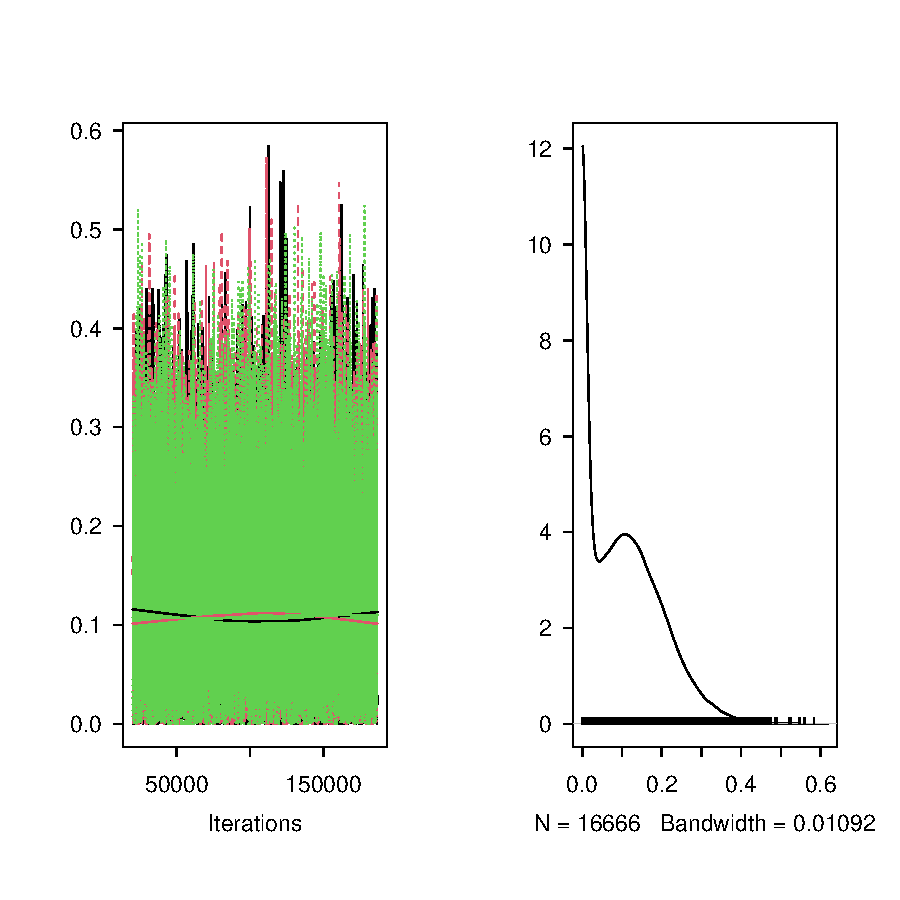
\includegraphics[width=.6\linewidth]{figure/FinalRFile-4350-Rnwauto-report-23} 

}


\begin{kframe}\begin{alltt}
\hlkwd{median}\hlstd{(mcmcChain[,}\hlnum{39}\hlstd{])}
\end{alltt}
\begin{verbatim}
## [1] 0.1046559
\end{verbatim}
\begin{alltt}
\hlkwd{mean}\hlstd{(mcmcChain[,}\hlnum{3}\hlstd{])}
\end{alltt}
\begin{verbatim}
## [1] 3.497763
\end{verbatim}
\begin{alltt}
\hlkwd{mean}\hlstd{(mcmcChain[,}\hlnum{9}\hlstd{])}
\end{alltt}
\begin{verbatim}
## [1] -5.840245
\end{verbatim}
\begin{alltt}
\hlkwd{mean}\hlstd{(mcmcChain[,}\hlnum{35}\hlstd{])}
\end{alltt}
\begin{verbatim}
## [1] -9.344268
\end{verbatim}
\end{kframe}
\end{knitrout}

The R session information (including the OS info, R version and all
packages used):

\begin{knitrout}
\definecolor{shadecolor}{rgb}{0.969, 0.969, 0.969}\color{fgcolor}\begin{kframe}
\begin{alltt}
\hlkwd{sessionInfo}\hlstd{()}
\end{alltt}
\begin{verbatim}
## R version 4.0.2 (2020-06-22)
## Platform: x86_64-apple-darwin17.0 (64-bit)
## Running under: macOS Catalina 10.15.5
## 
## Matrix products: default
## BLAS:   /System/Library/Frameworks/Accelerate.framework/Versions/A/Frameworks/vecLib.framework/Versions/A/libBLAS.dylib
## LAPACK: /Library/Frameworks/R.framework/Versions/4.0/Resources/lib/libRlapack.dylib
## 
## locale:
## [1] en_US.UTF-8/en_US.UTF-8/en_US.UTF-8/C/en_US.UTF-8/en_US.UTF-8
## 
## attached base packages:
## [1] stats     graphics  grDevices utils     datasets  methods   base     
## 
## other attached packages:
## [1] knitr_1.29      bayesplot_1.8.0 MCMCvis_0.15.0  rjags_4-10      coda_0.19-4    
## [6] ggplot2_3.3.3  
## 
## loaded via a namespace (and not attached):
##  [1] Rcpp_1.0.5       highr_0.8        pillar_1.4.6     compiler_4.0.2   plyr_1.8.6      
##  [6] tools_4.0.2      digest_0.6.25    evaluate_0.14    lifecycle_0.2.0  tibble_3.0.3    
## [11] gtable_0.3.0     lattice_0.20-41  pkgconfig_2.0.3  rlang_0.4.7      rstudioapi_0.11 
## [16] xfun_0.16        withr_2.2.0      dplyr_1.0.2      stringr_1.4.0    generics_0.1.0  
## [21] vctrs_0.3.4      grid_4.0.2       tidyselect_1.1.0 glue_1.4.2       R6_2.4.1        
## [26] farver_2.0.3     purrr_0.3.4      reshape2_1.4.4   magrittr_1.5     scales_1.1.1    
## [31] ggridges_0.5.3   ellipsis_0.3.1   colorspace_1.4-1 labeling_0.3     tinytex_0.25    
## [36] stringi_1.4.6    munsell_0.5.0    crayon_1.3.4
\end{verbatim}
\begin{alltt}
\hlkwd{Sys.time}\hlstd{()}
\end{alltt}
\begin{verbatim}
## [1] "2021-05-05 11:39:36 EDT"
\end{verbatim}
\end{kframe}
\end{knitrout}


\end{document}
